%\chapter{Results \& Discussion}
%
%In this chapter a number of visualizations are presented, however the full list of visualizations, around 70 can be found in the appendix.
%
%\section{Data Collection Validation}
%
%In the pre-processing experiment, the method used for collecting and filtering the 1000 Tweets.
%To test that the distribution and collection was being done correctly, figures~\ref{fig:preprocessdist} and~\ref{fig:finaldist} where generated.
%
%
%\begin{figure}[!htb]
%\minipage{0.5\textwidth}
%  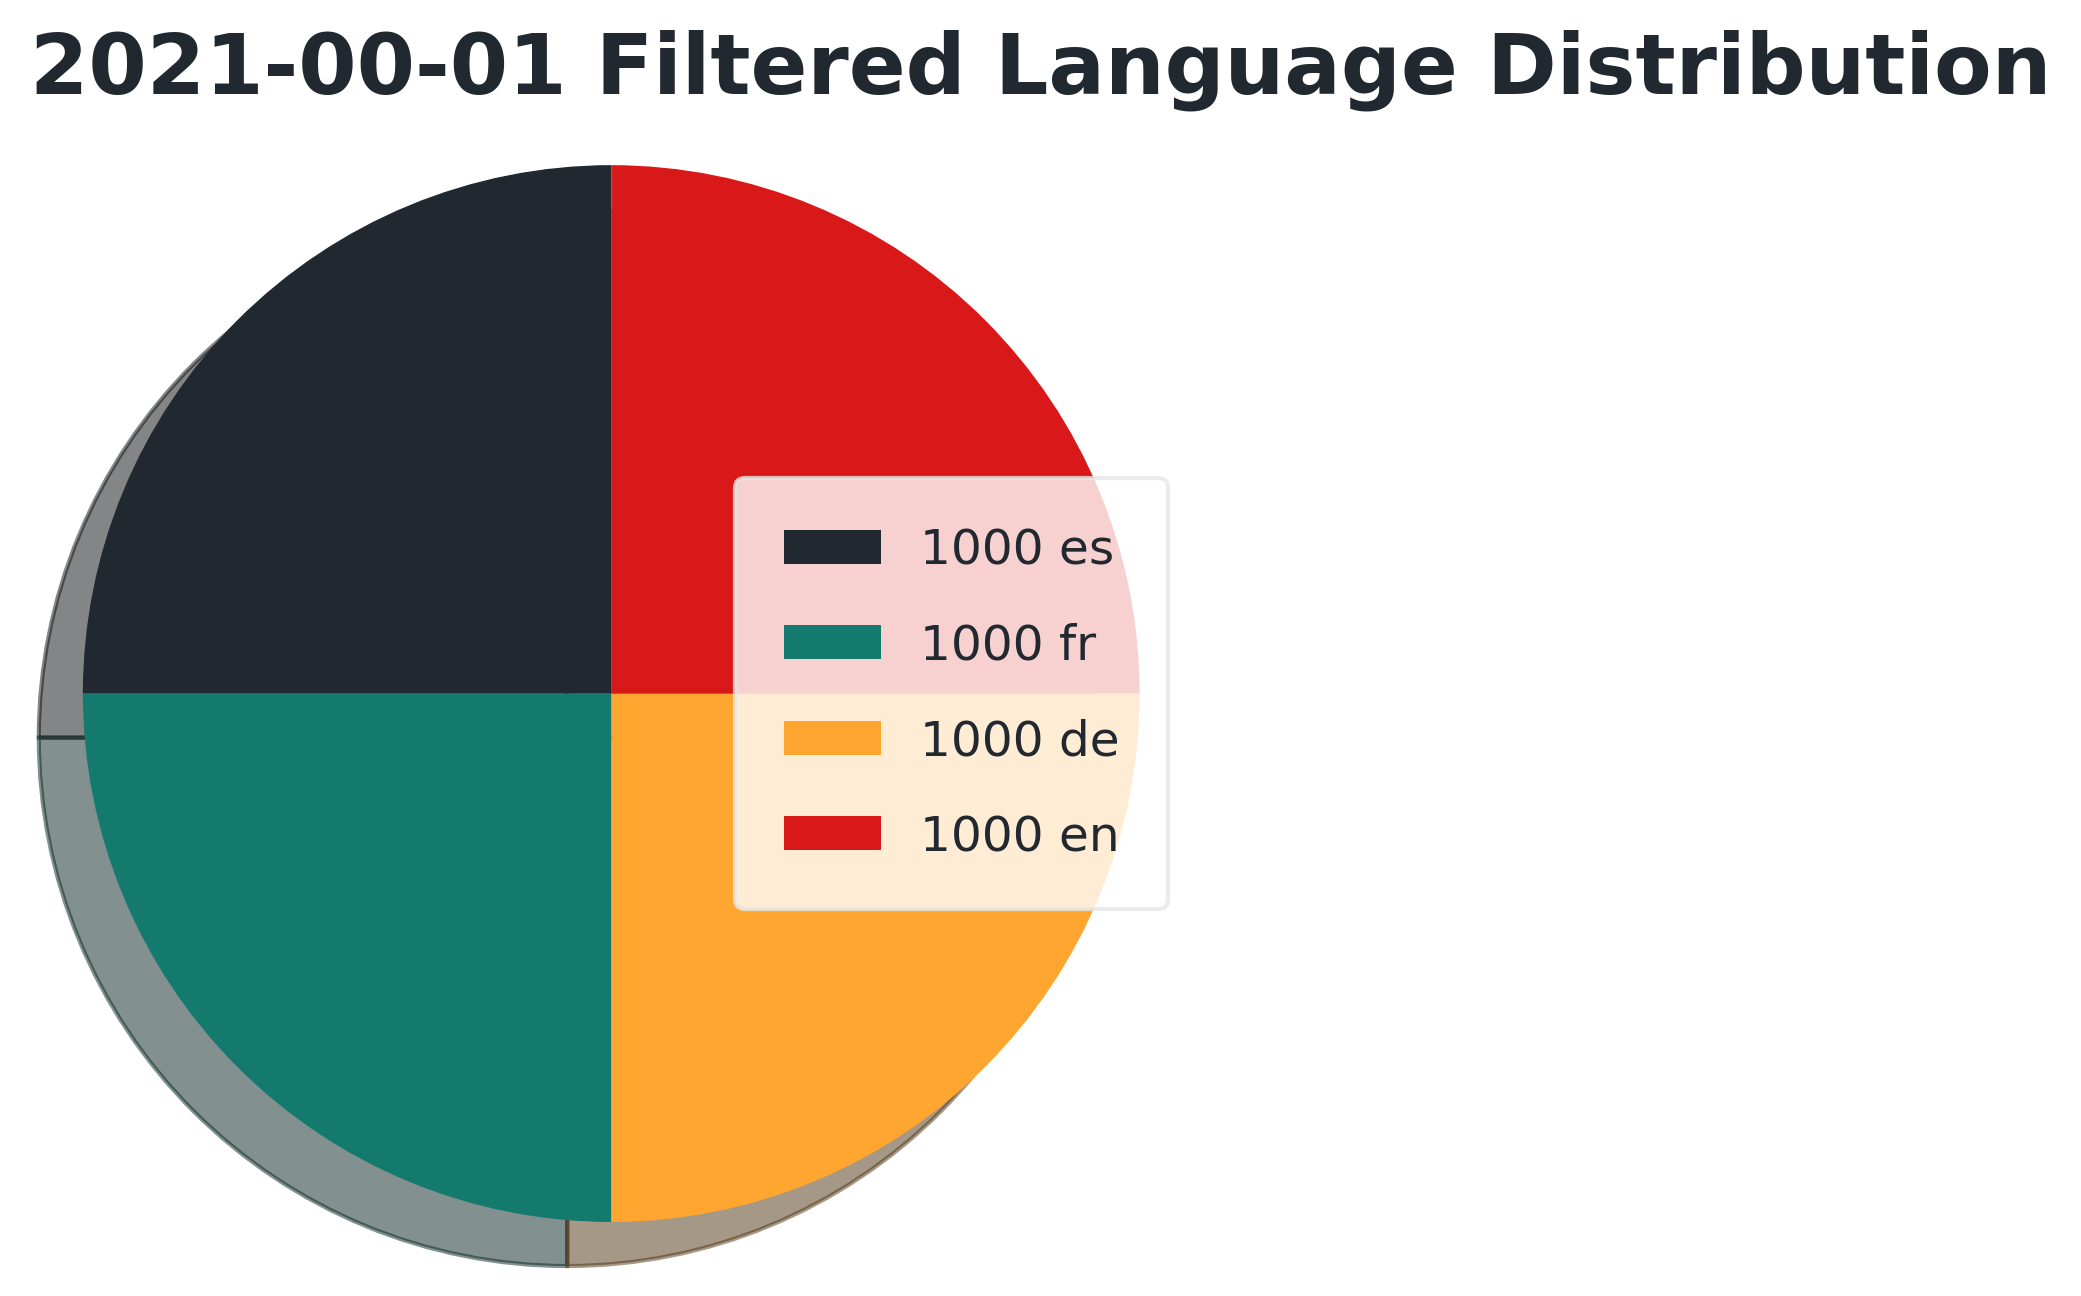
\includegraphics[width=\linewidth]{2021-00-01 Filtered Language Distribution.png}
%  \caption[Pre-Process Filtered Language Distribution]{ }
%  \label{fig:preprocessdist}
%\endminipage\hfill
%\minipage{0.5\textwidth}
%  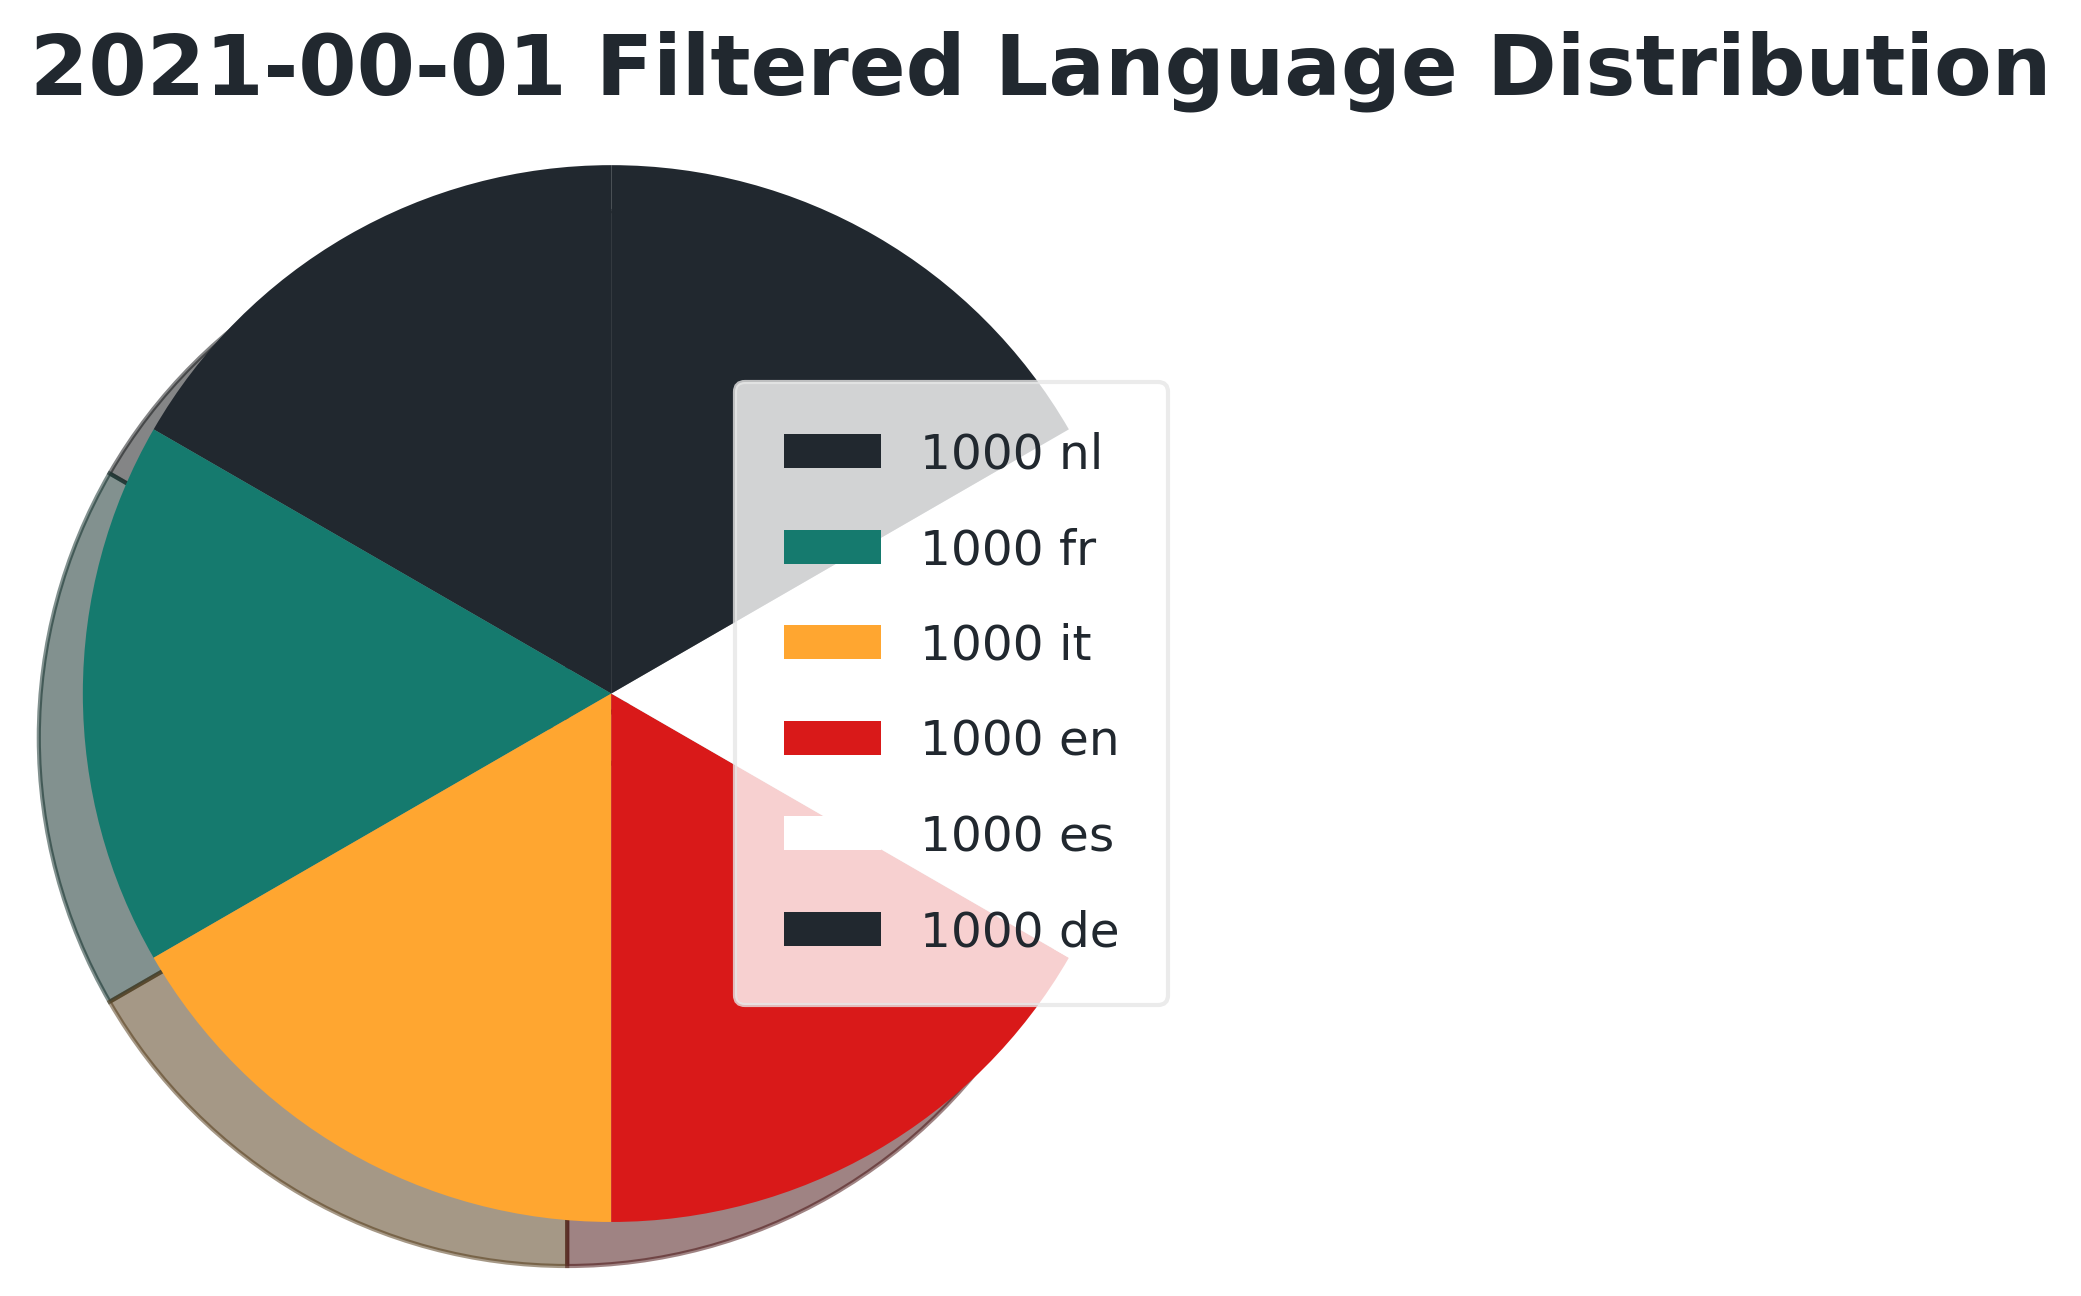
\includegraphics[width=\linewidth]{2021-01-01 Filtered Language Distribution - Final.png}
%  \caption[Final Filtered Language Distribution]{ }
%  \label{fig:finaldist}
%\endminipage
%\end{figure}
%
%
%\section{Pre-Processing Effect}
%
%The compound sentiment scores returned from the \ac{VADER} model was averaged and plotted for the 3 dates used in the experiment.
%The 4 graphs produced, figures~\ref{fig:EnglishPre} to~\ref{fig:GermanPre}, show a time series graph of each language over the 3 days which are 1 month apart.
%The mean scores where also summed and the difference between the pre-processed and non-processed total was of 0.17\%.
%
%\begin{figure}[!htb]
%\minipage{0.5\textwidth}
%  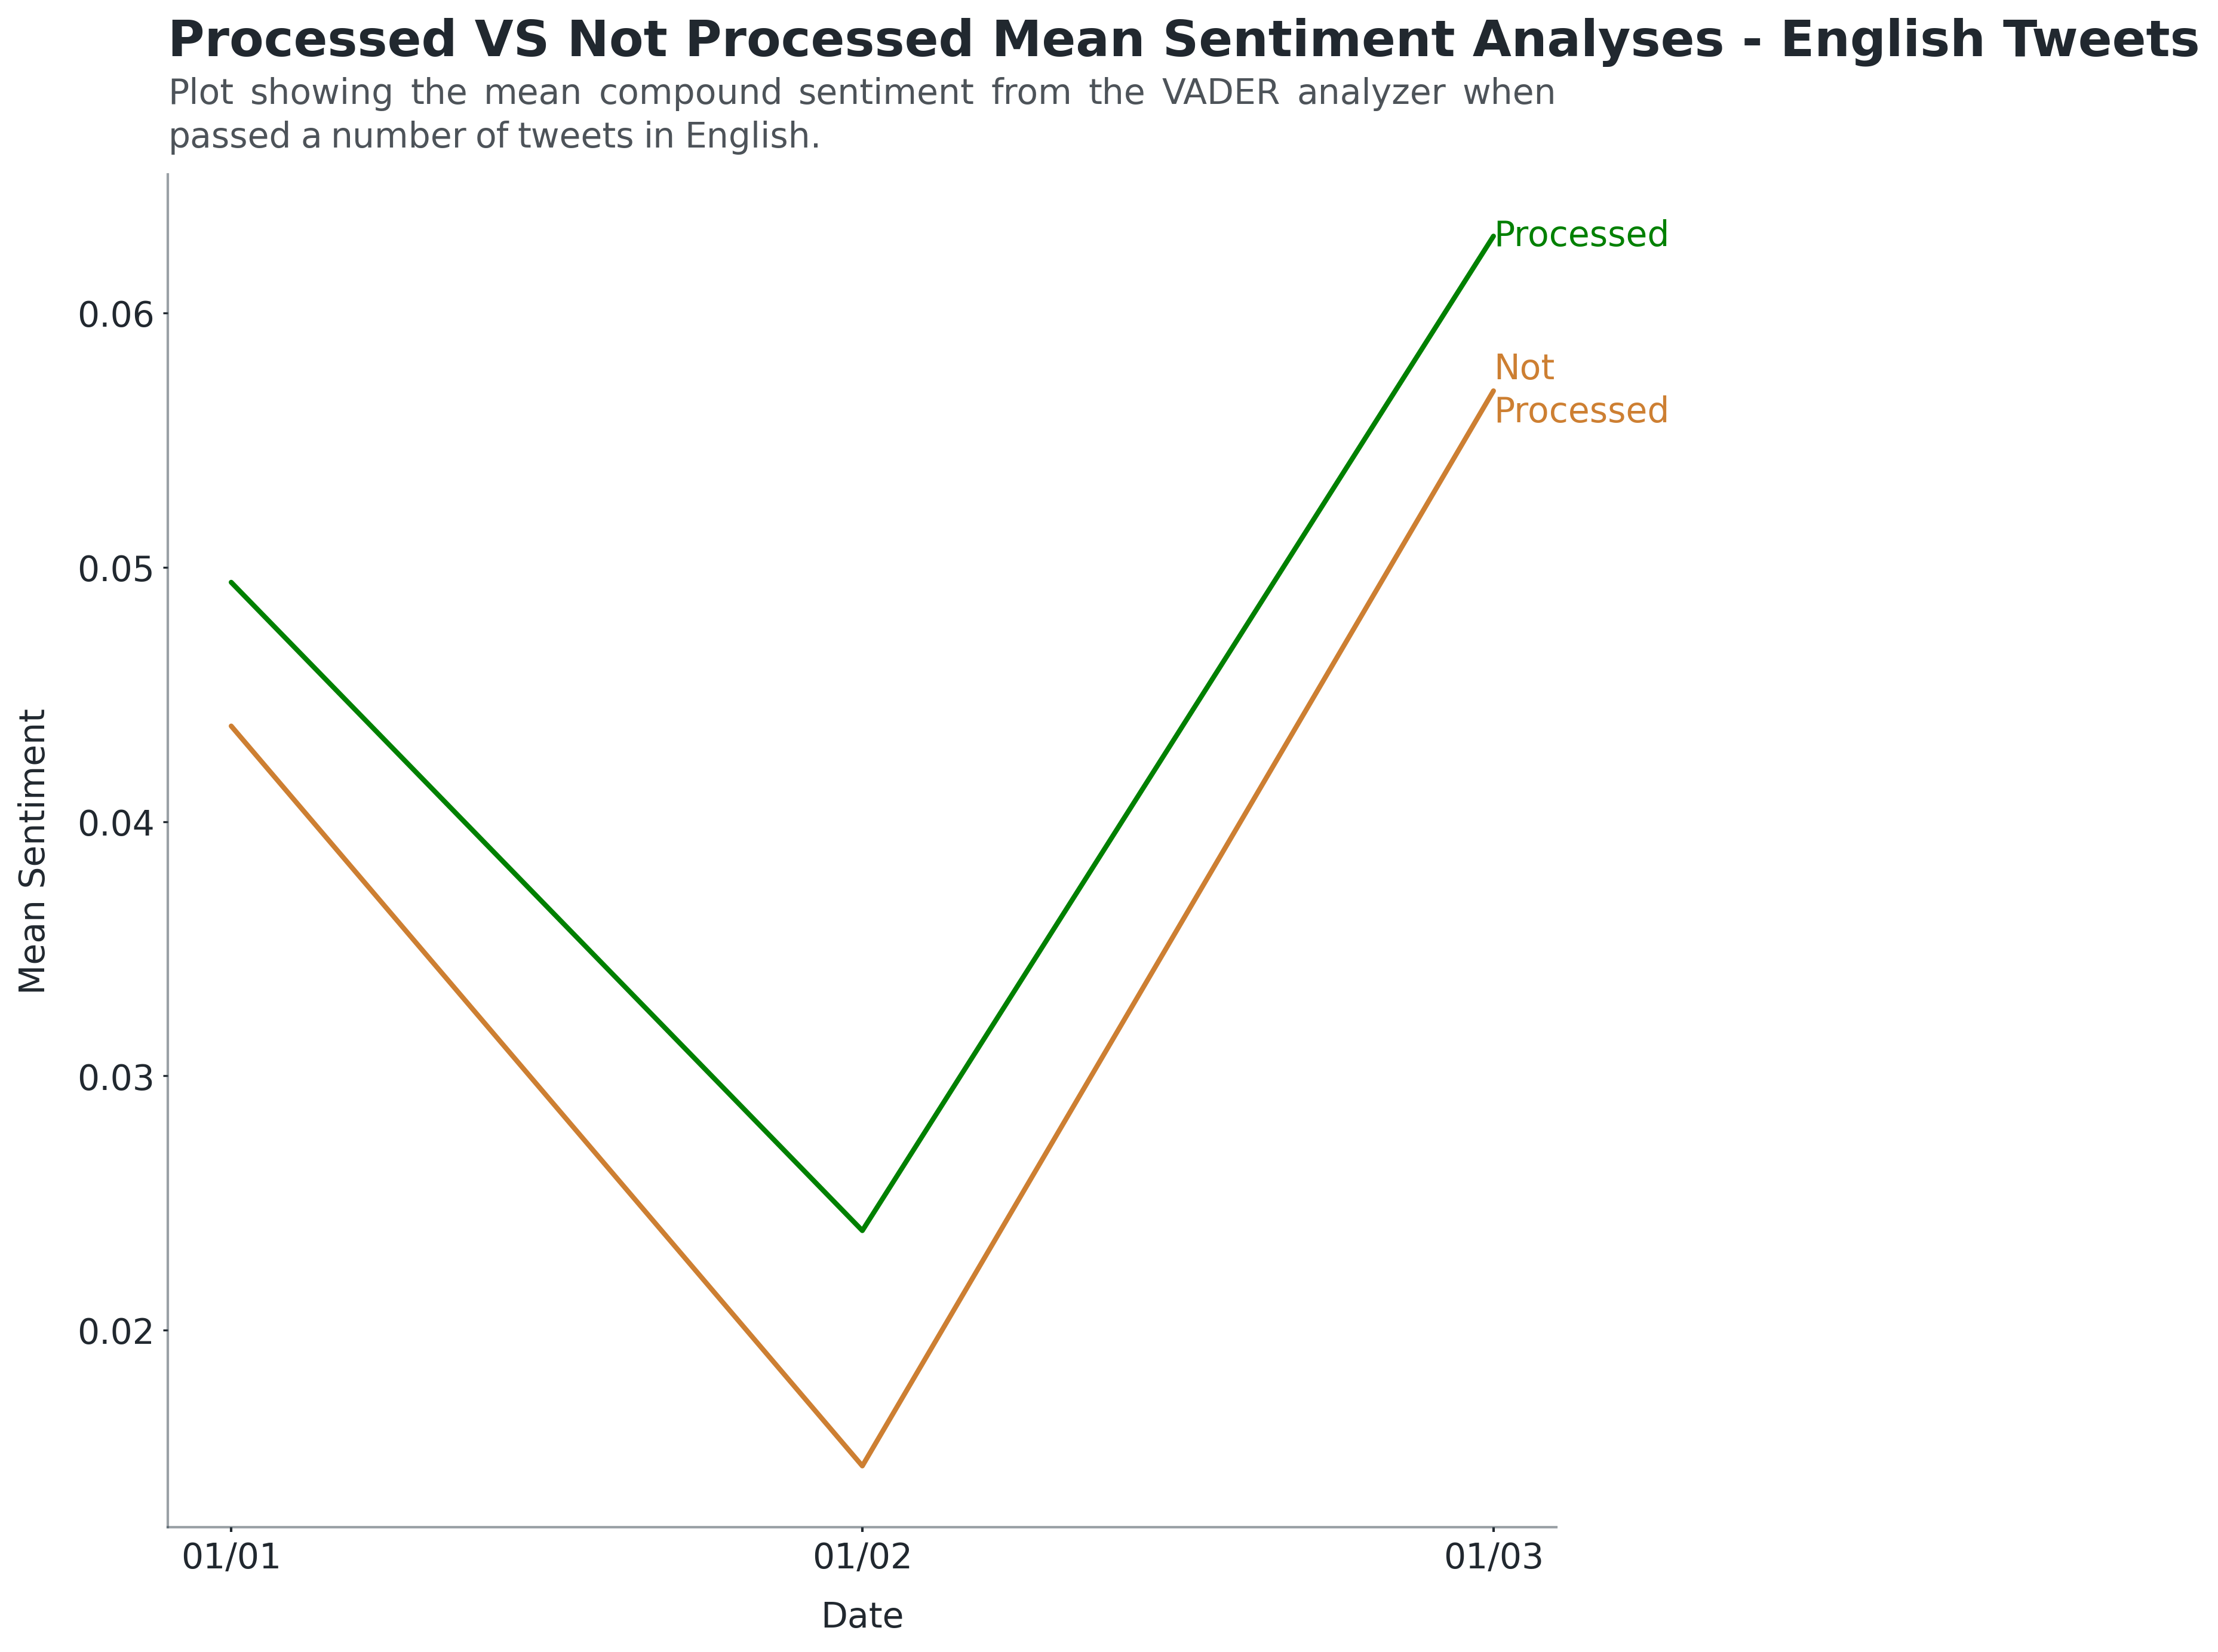
\includegraphics[width=\linewidth]{English Process VS NotProcessed.png}
%  \caption[English Process VS NotProcessed]{ }\label{fig:EnglishPre}
%\endminipage\hfill
%\minipage{0.5\textwidth}
%  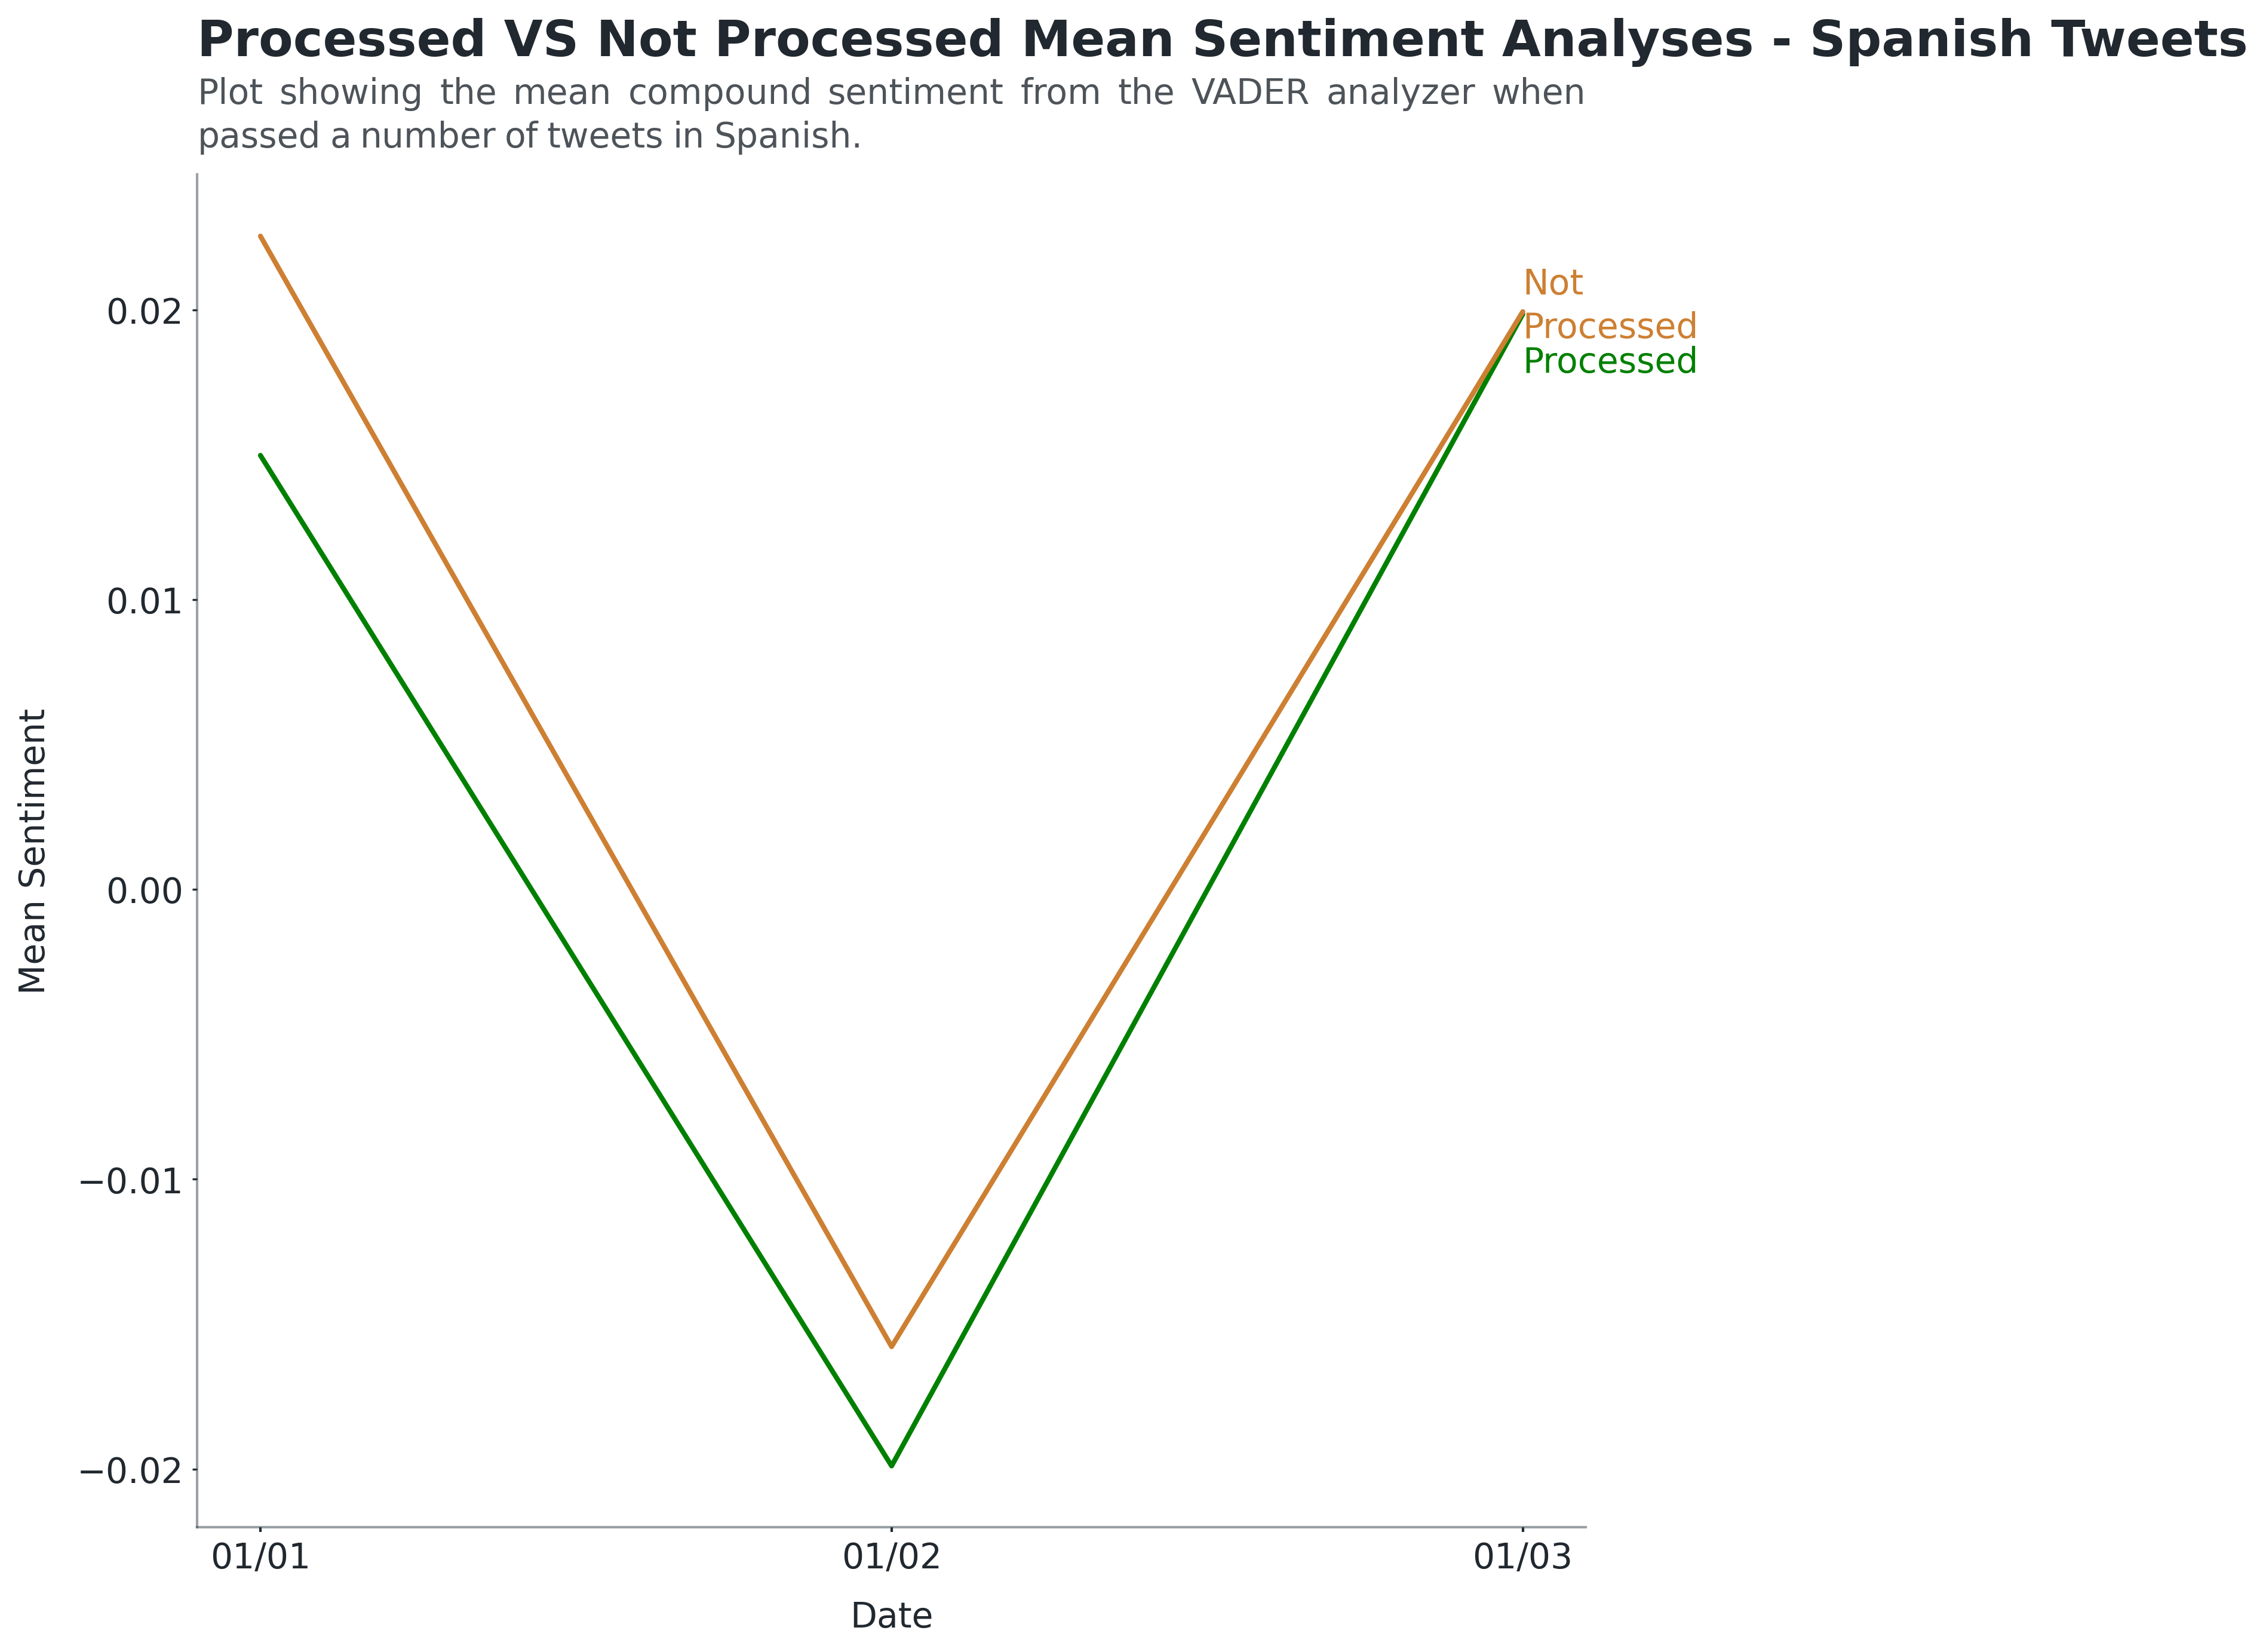
\includegraphics[width=\linewidth]{Spanish Process VS NotProcessed.png}
%  \caption[Spanish Process VS NotProcessed]{ }\label{fig:SpanishPre}
%\endminipage
%\end{figure}
%\begin{figure}[!htb]
%\minipage{0.5\textwidth}
%  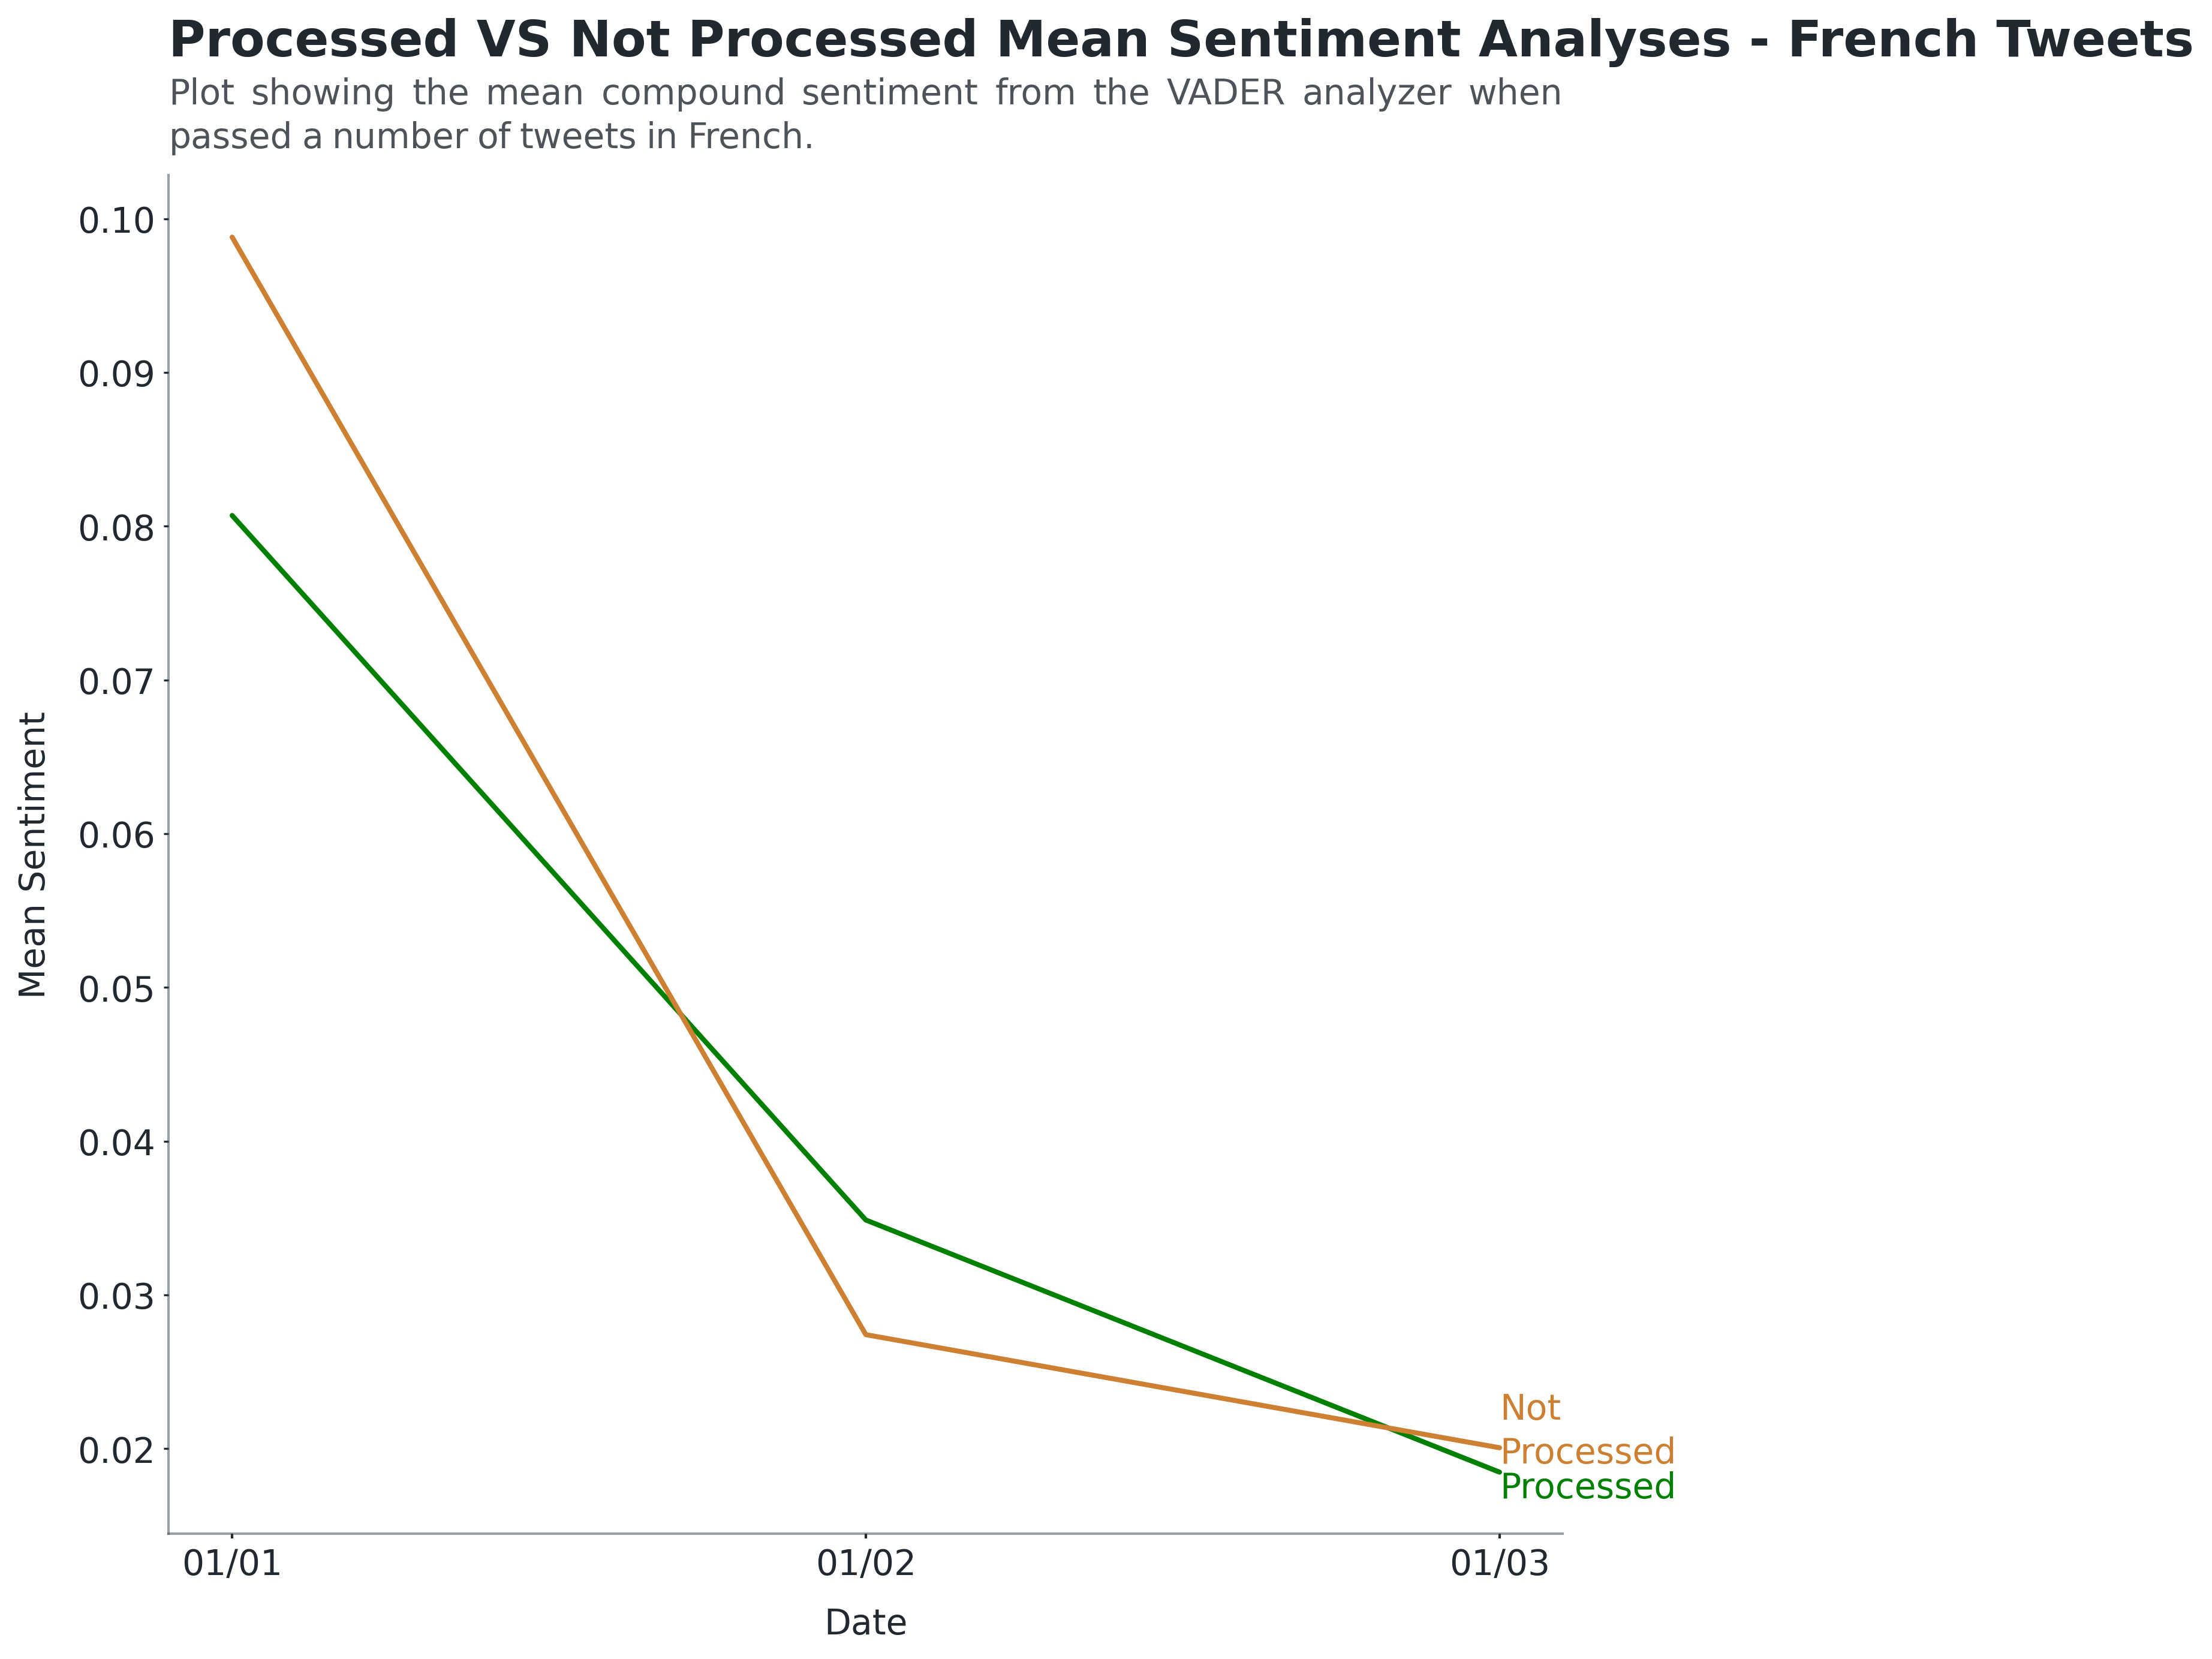
\includegraphics[width=\linewidth]{French Process VS NotProcessed.png}
%  \caption[French Process VS NotProcessed]{ }\label{fig:FrenchPre}
%\endminipage\hfill
%\minipage{0.5\textwidth}
%  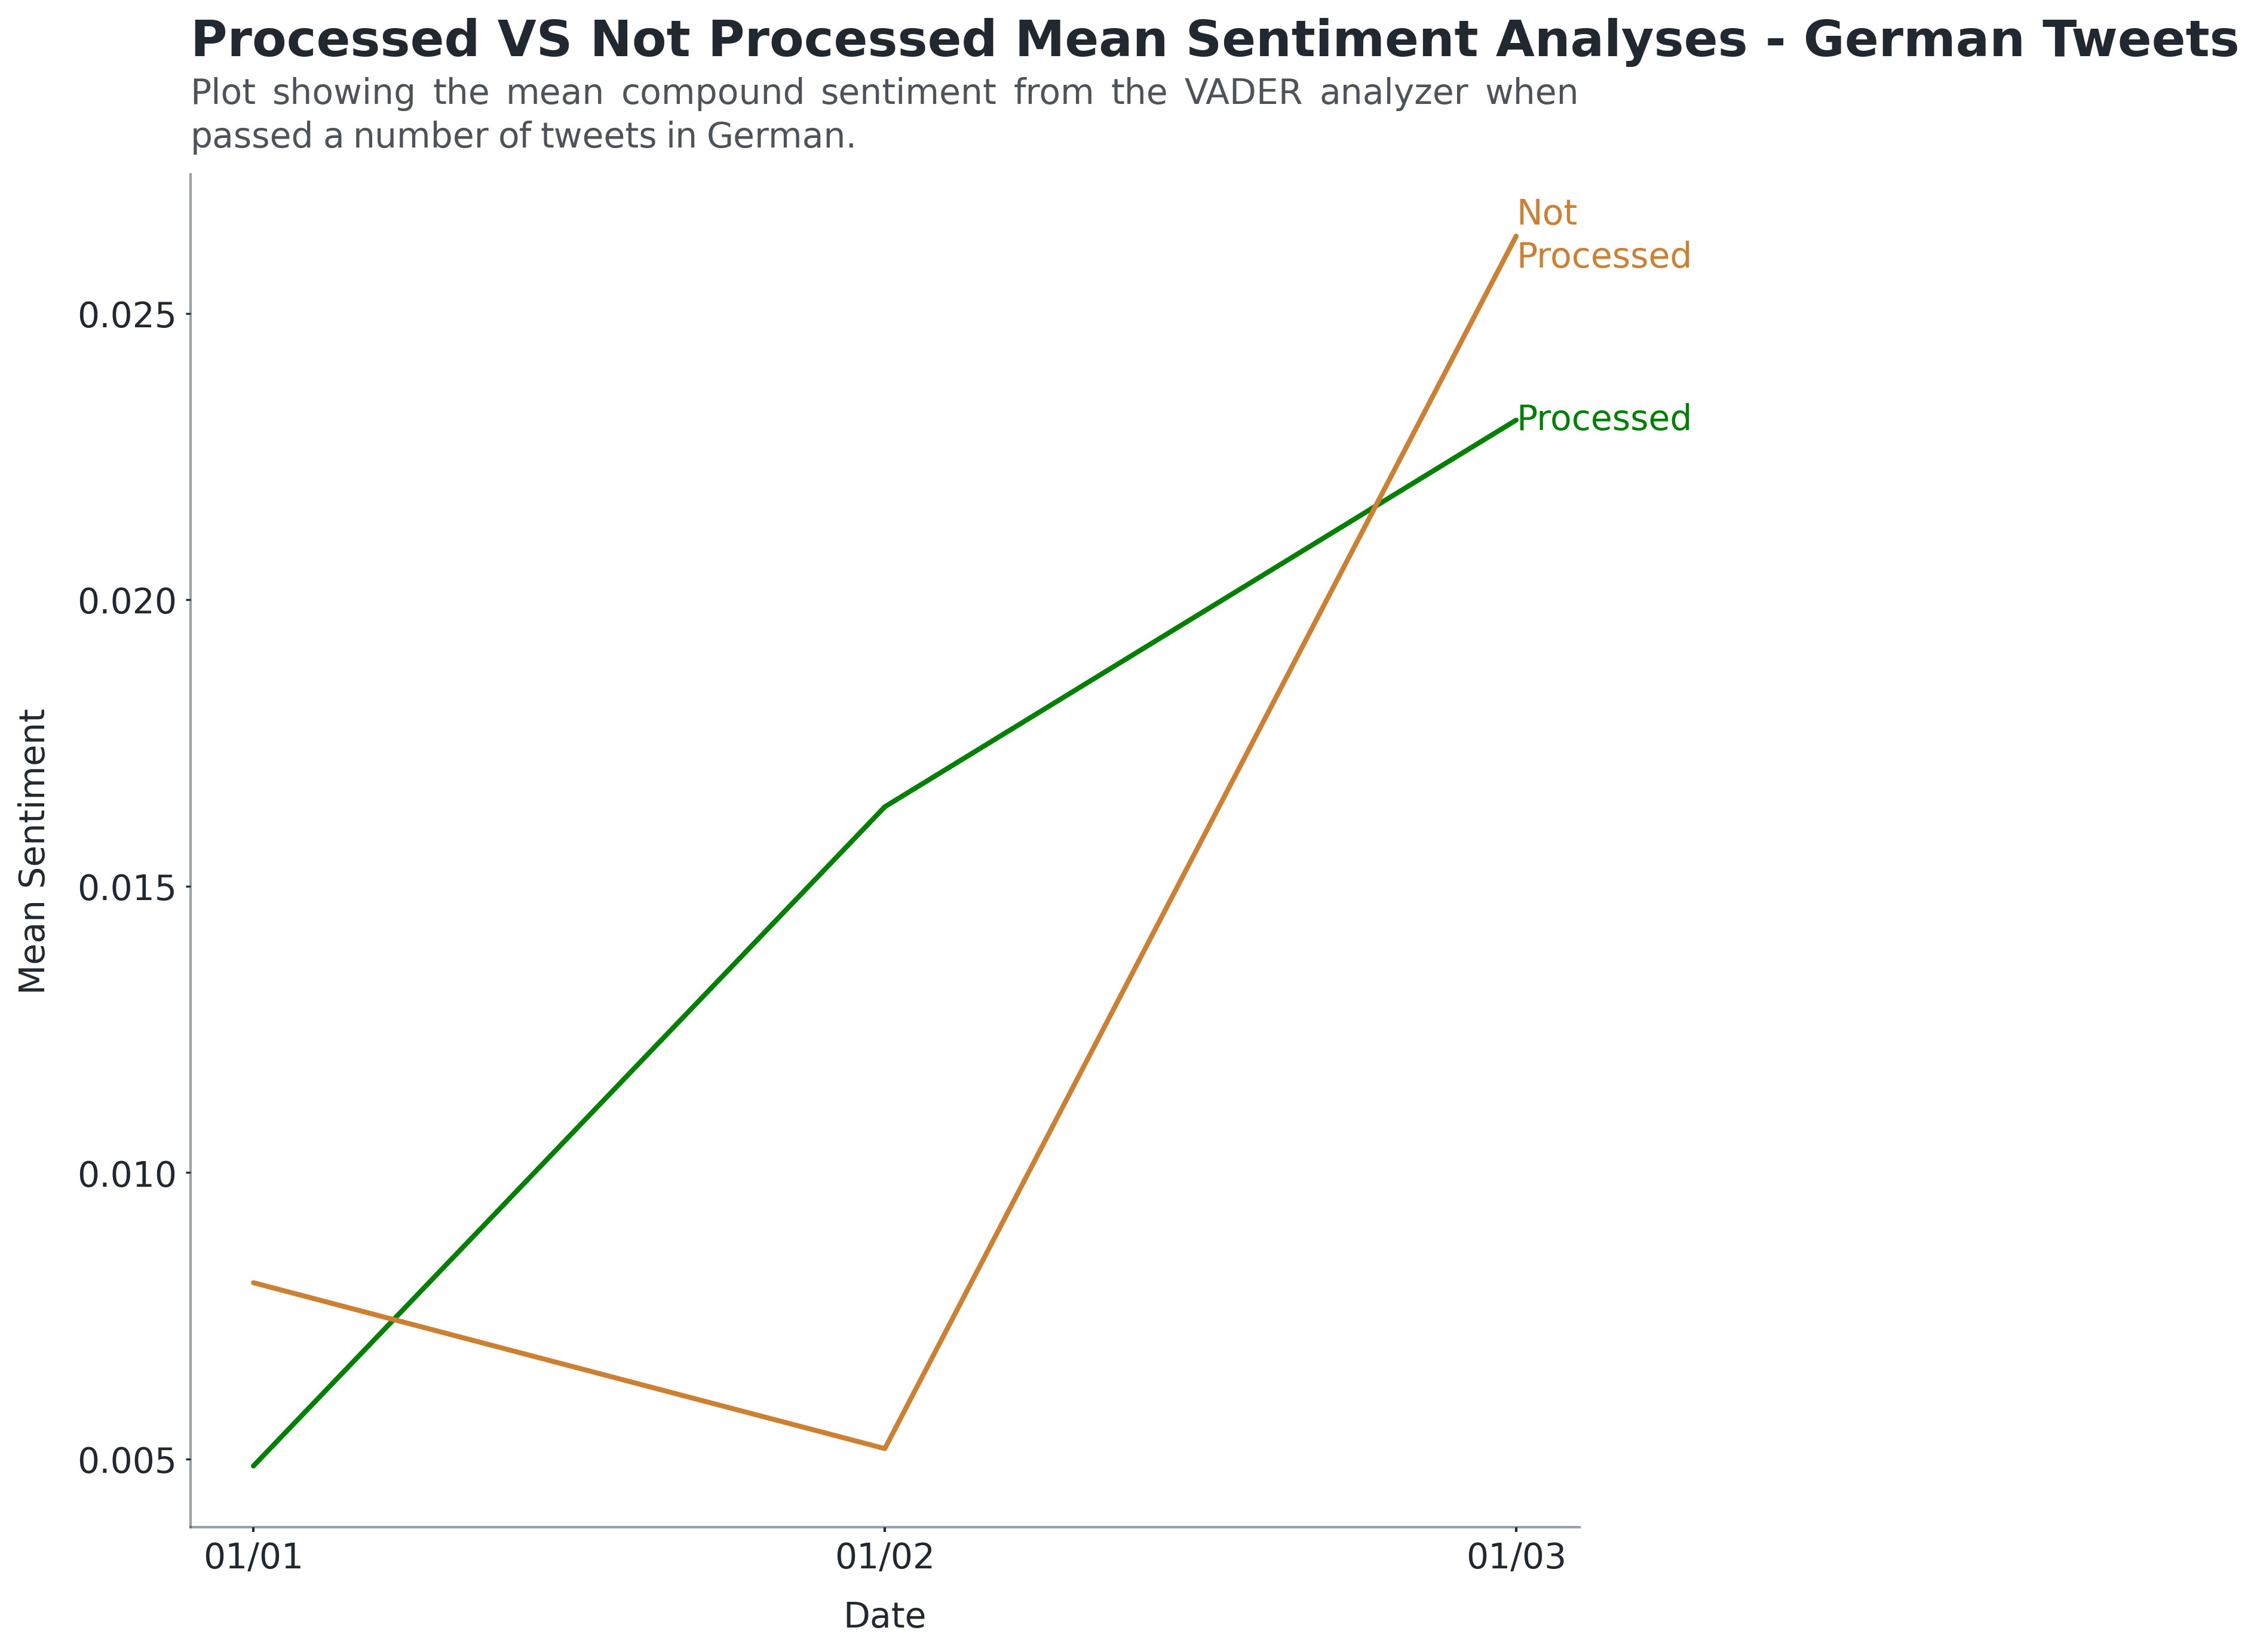
\includegraphics[width=\linewidth]{German Process VS NotProcessed.png}
%  \caption[German Process VS NotProcessed]{ }\label{fig:GermanPre}
%\endminipage
%\end{figure}
%
%\noindent The difference calculated along with the shapes of the graphs plotted were not considered significant enough to remove pre-processing.
%However the pre-process function was amended to keep more features like emojis and hashtags, which prior to this experiment where being removed.
%
%\section{Daily Twitter Mean Sentiment}
%
%Just as with figures~\ref{fig:EnglishPre} to~\ref{fig:GermanPre}, time series graphs where plotted for the mean sentiment scores on the larger 180,000 tweet dataset.
%When all the languages are plotted against each other in figure~\ref{fig:globalall} show no clear trend, however some languages are closer to each other than others.
%When these languages are separated in figures~\ref{fig:globalmean} and~\ref{fig:globaleu} the mean of the compound scores can be seen to related more to each other.
%
%\begin{figure}[h!]
%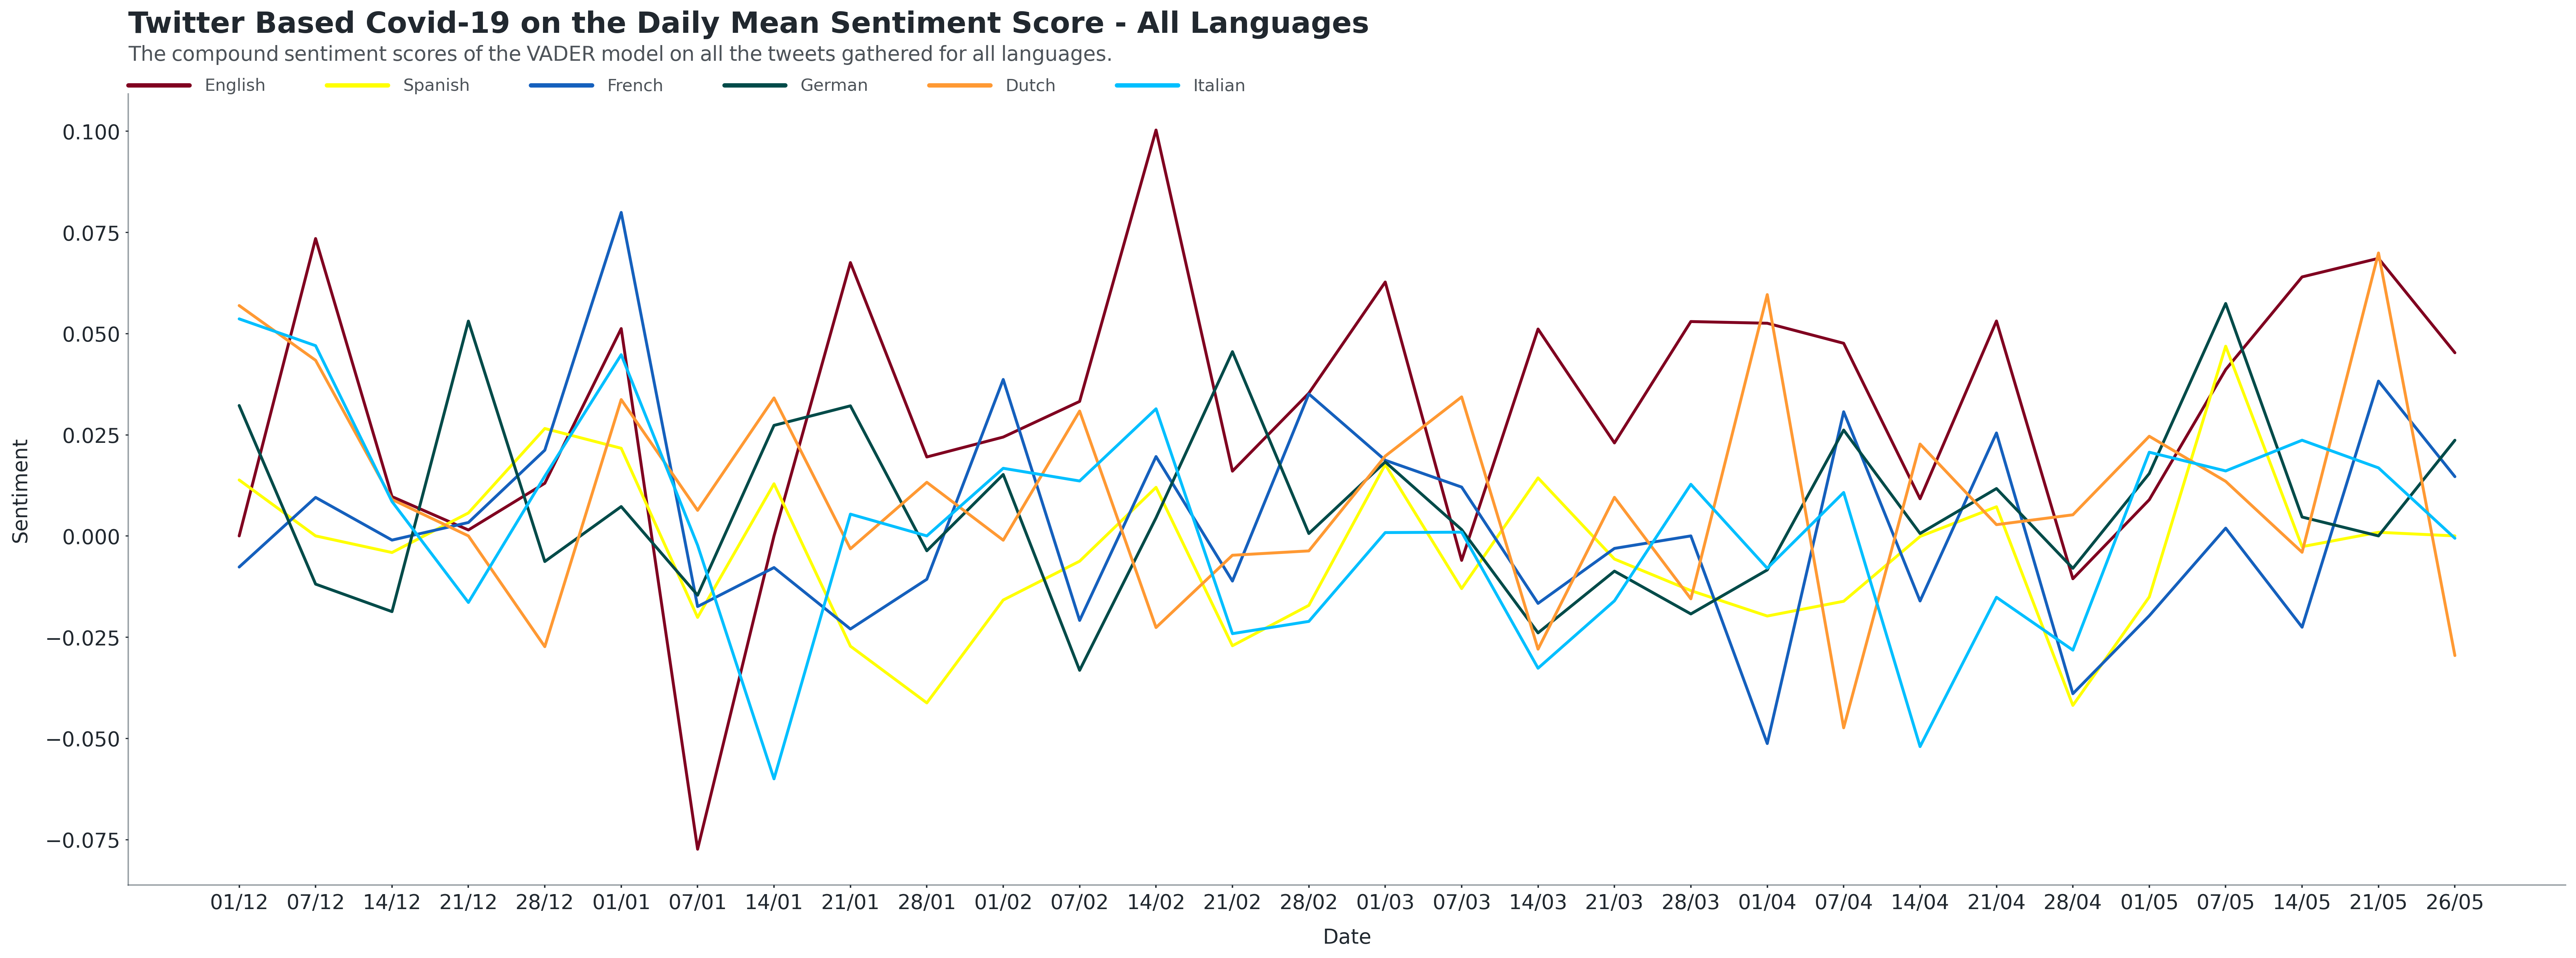
\includegraphics[scale=0.24]{Daily Mean All.png}
%\caption[Daily Mean All]{ }
%\label{fig:globalall}
%\end{figure}
%
%\noindent For figure~\ref{fig:globalall}, the effect of translation is very apparent with the reduced information given from the lines plotted from non-English tweets.
%
%\begin{figure}[h!]
%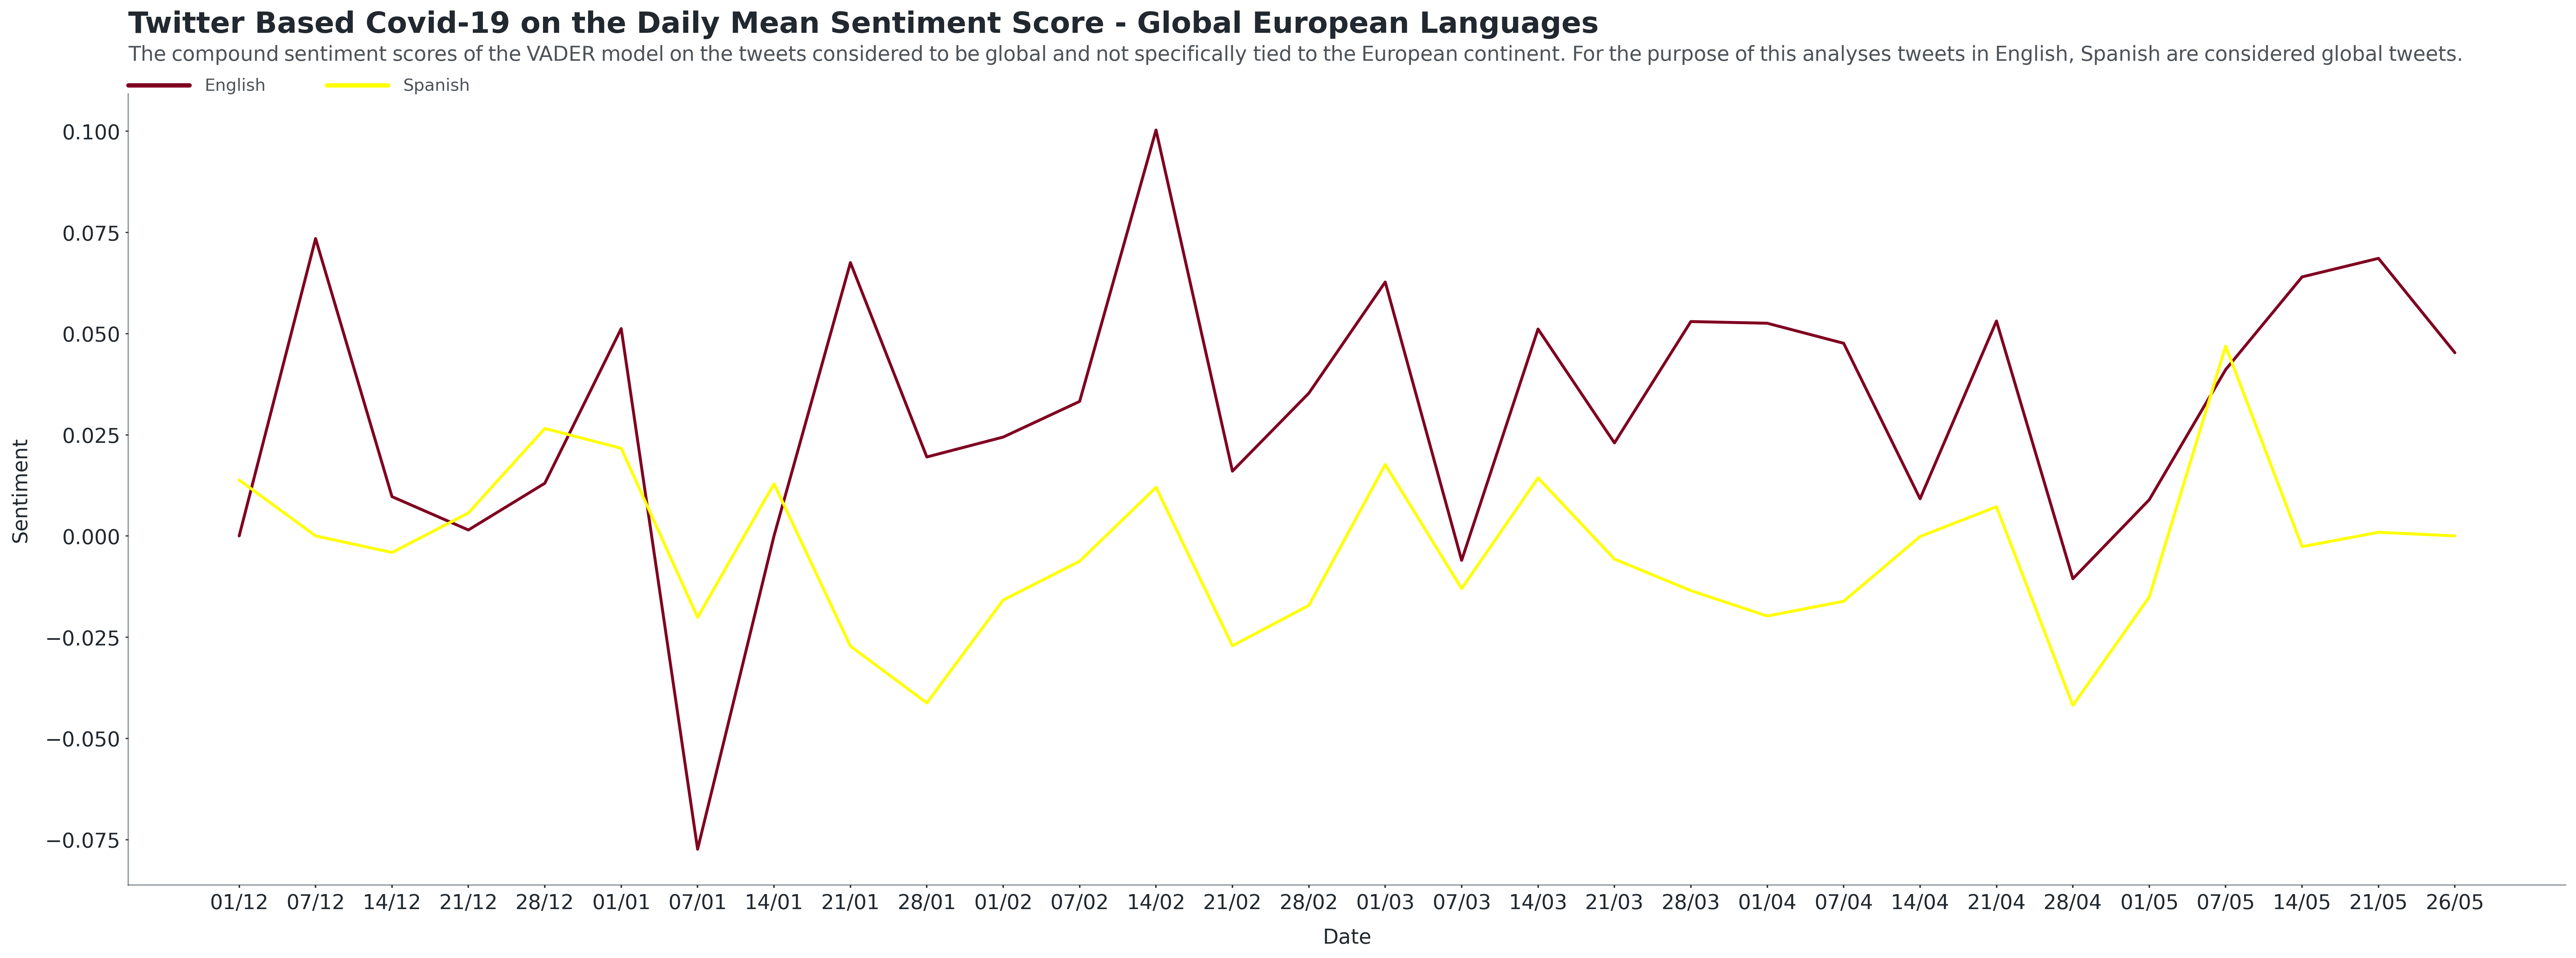
\includegraphics[scale=0.24]{Daily Mean Global.png}
%\caption[Daily Mean Global]{ }
%\label{fig:globalmean}
%\end{figure}
%
%\noindent For figure~\ref{fig:globalmean}, although not followed exactly, the shape of the Spanish line corresponds to the peaks and dips of the English line.
%
%\begin{figure}[h!]
%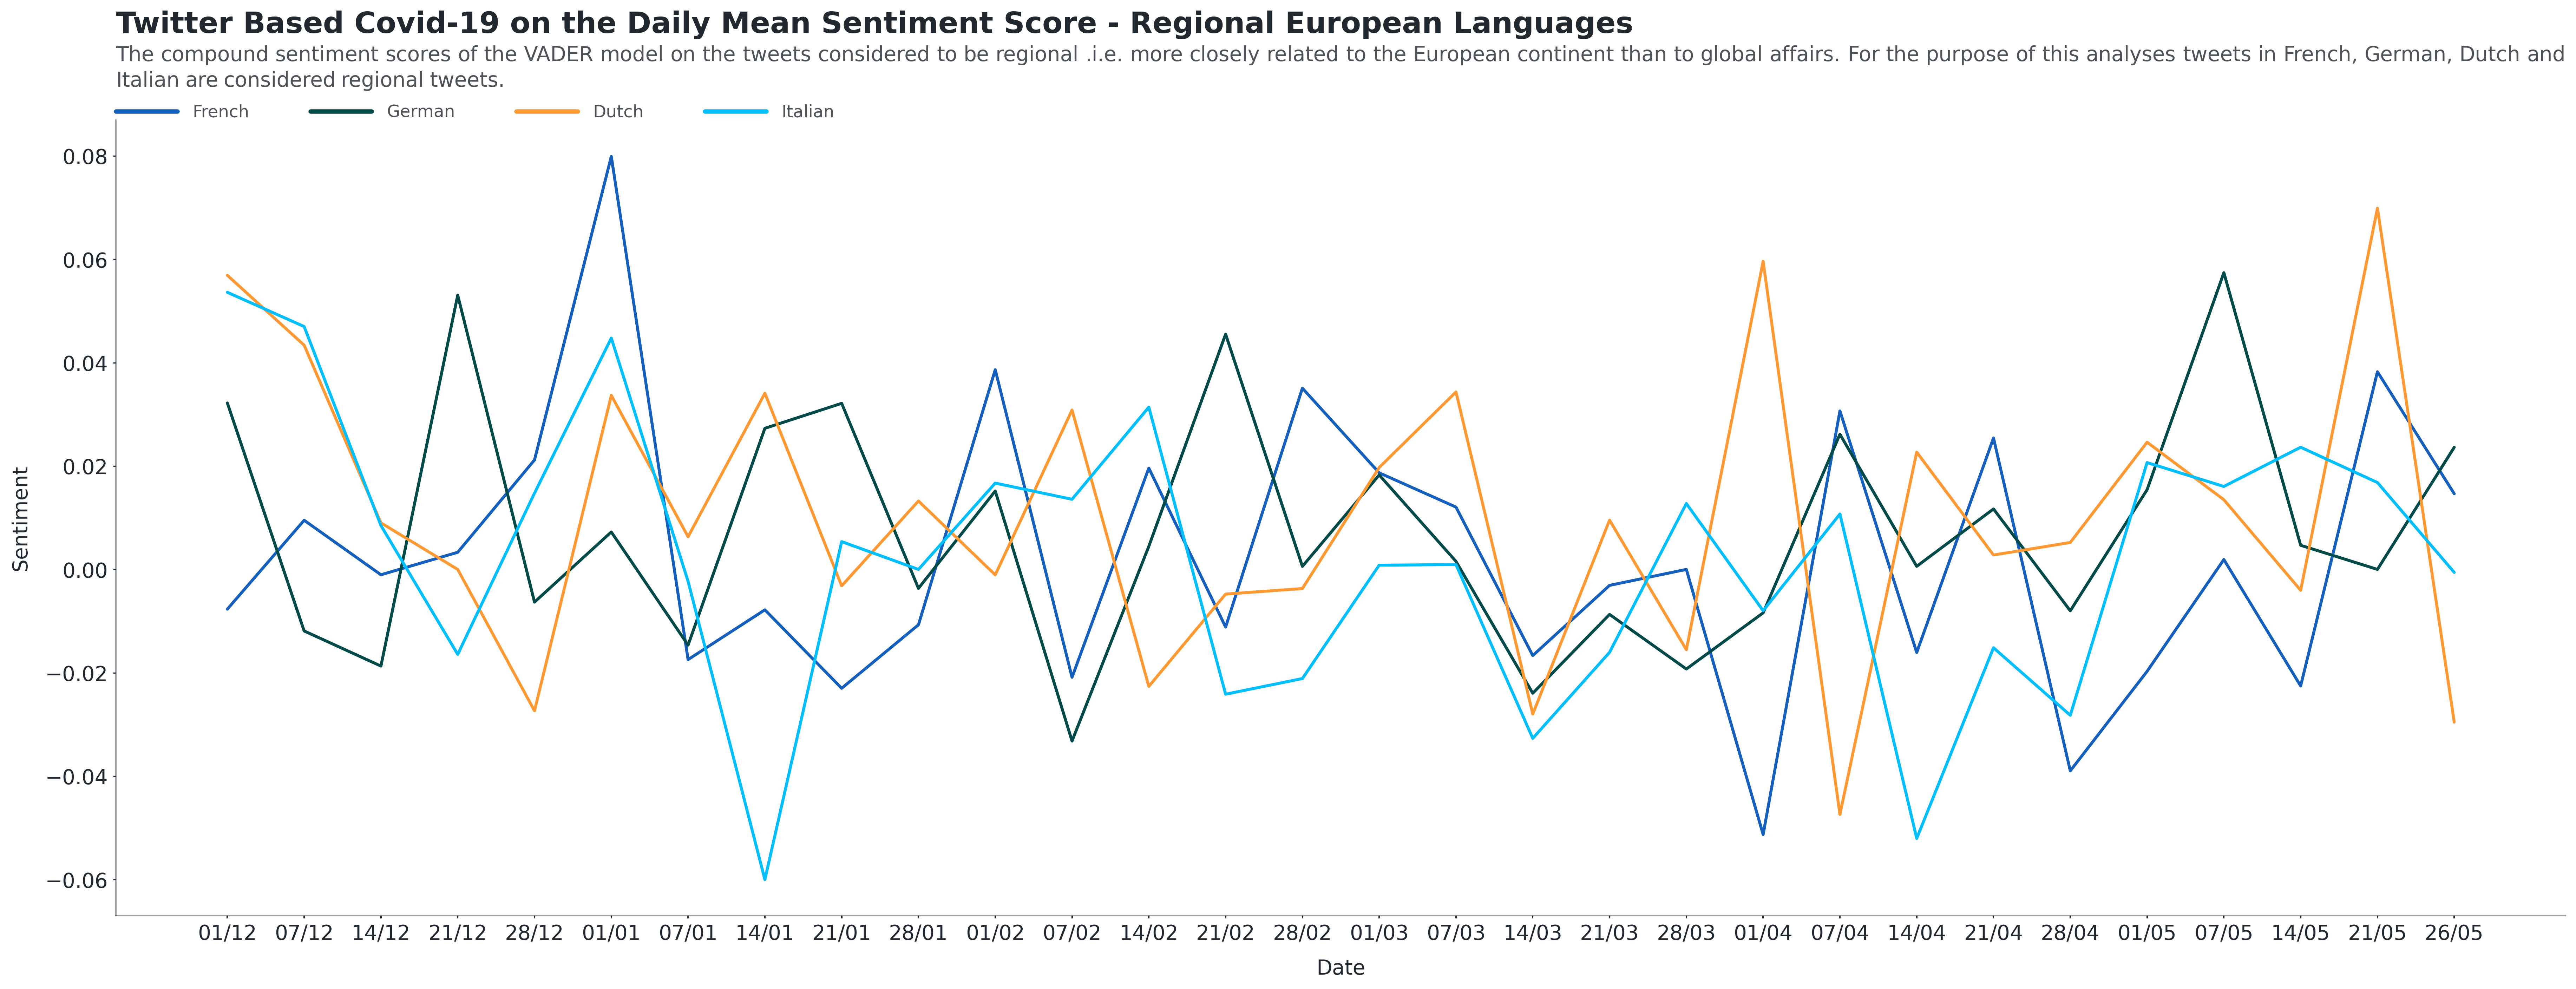
\includegraphics[scale=0.24]{Daily Mean Europe.png}
%\caption[Daily Mean Europe]{ }
%\label{fig:globaleu}
%\end{figure}
%
%\noindent For figure~\ref{fig:globaleu}, the line plots for these languages where expected to be more closely related however some similarities can be seen.
%On holidays such as 1st January (new years) or 14th February(valentines day) most countries experience a peak in positivity.
%Inversely on the 14th March every country experienced a dip in positivity.
%
%\section{Daily Twitter Sentiment Classification}
%
%By classifying each compound score in a positivity class, a time series plot is plotted for each country can better visualize the changes sentiment over time.
%Article headings and tweets annotated to dips and peaks of the lines in the plot to represent a random snippet of what was being said on that day.
%
%\begin{figure}[h!]
%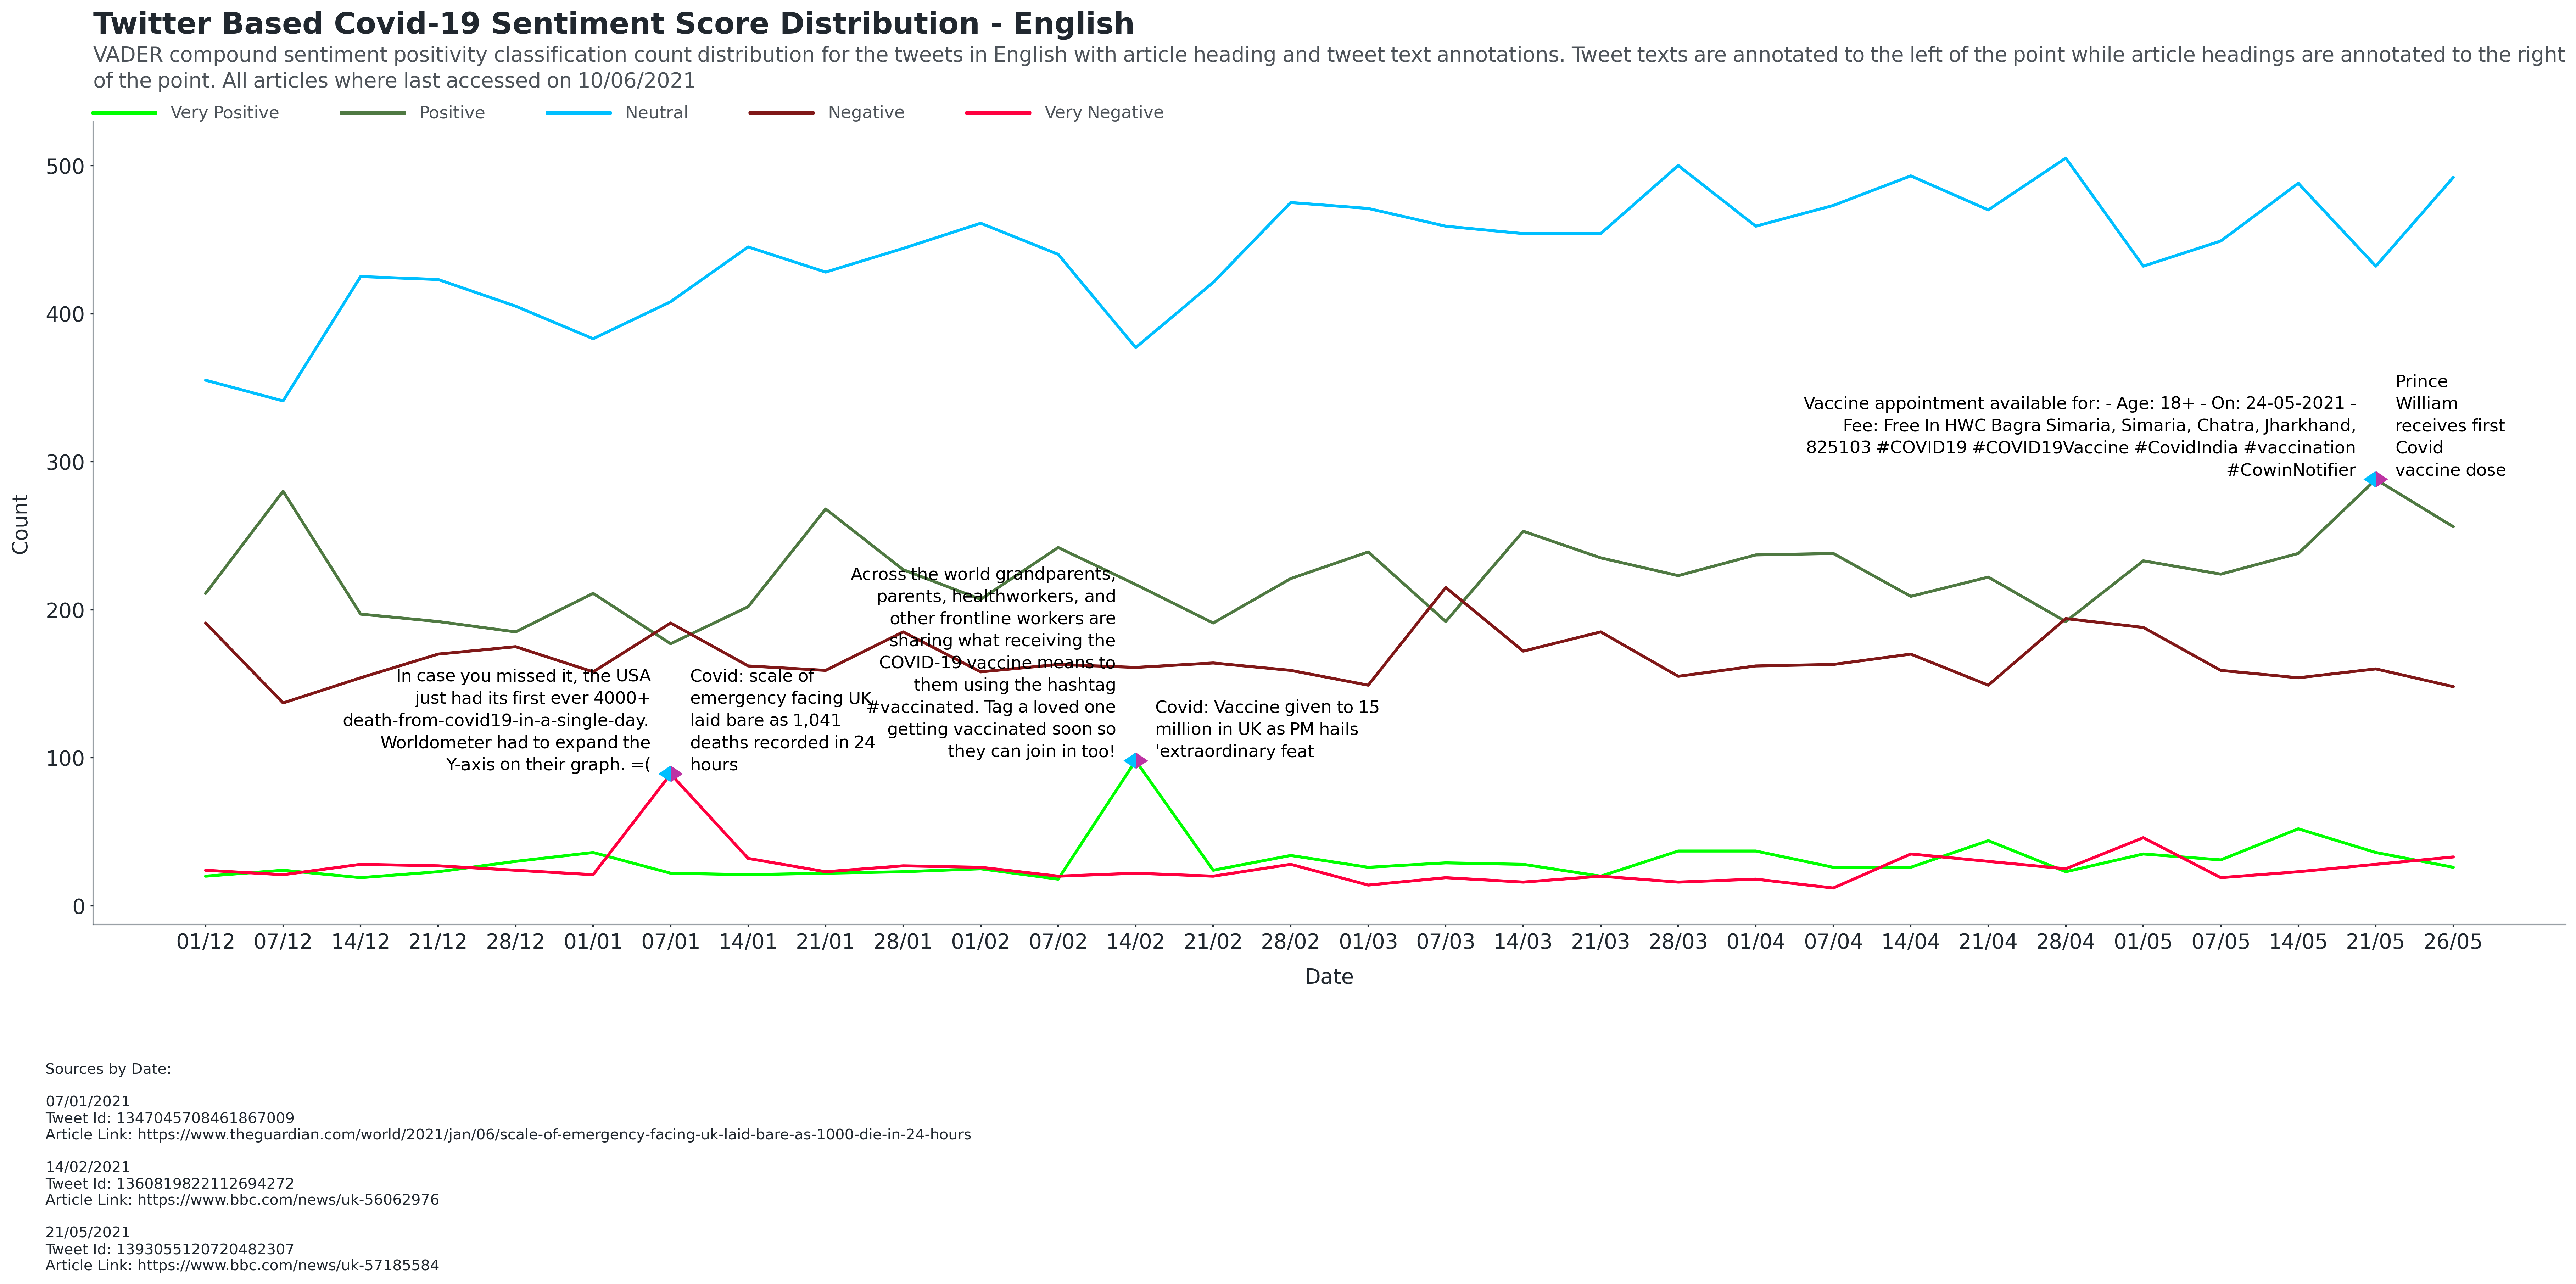
\includegraphics[scale=0.24]{Final English Annotated Distribution.png}
%\caption[English Annotated Sentiment Distribution]{ }
%\label{fig:English}
%\end{figure}
%
%\newpage
%%
%%\begin{figure}[h!]
%%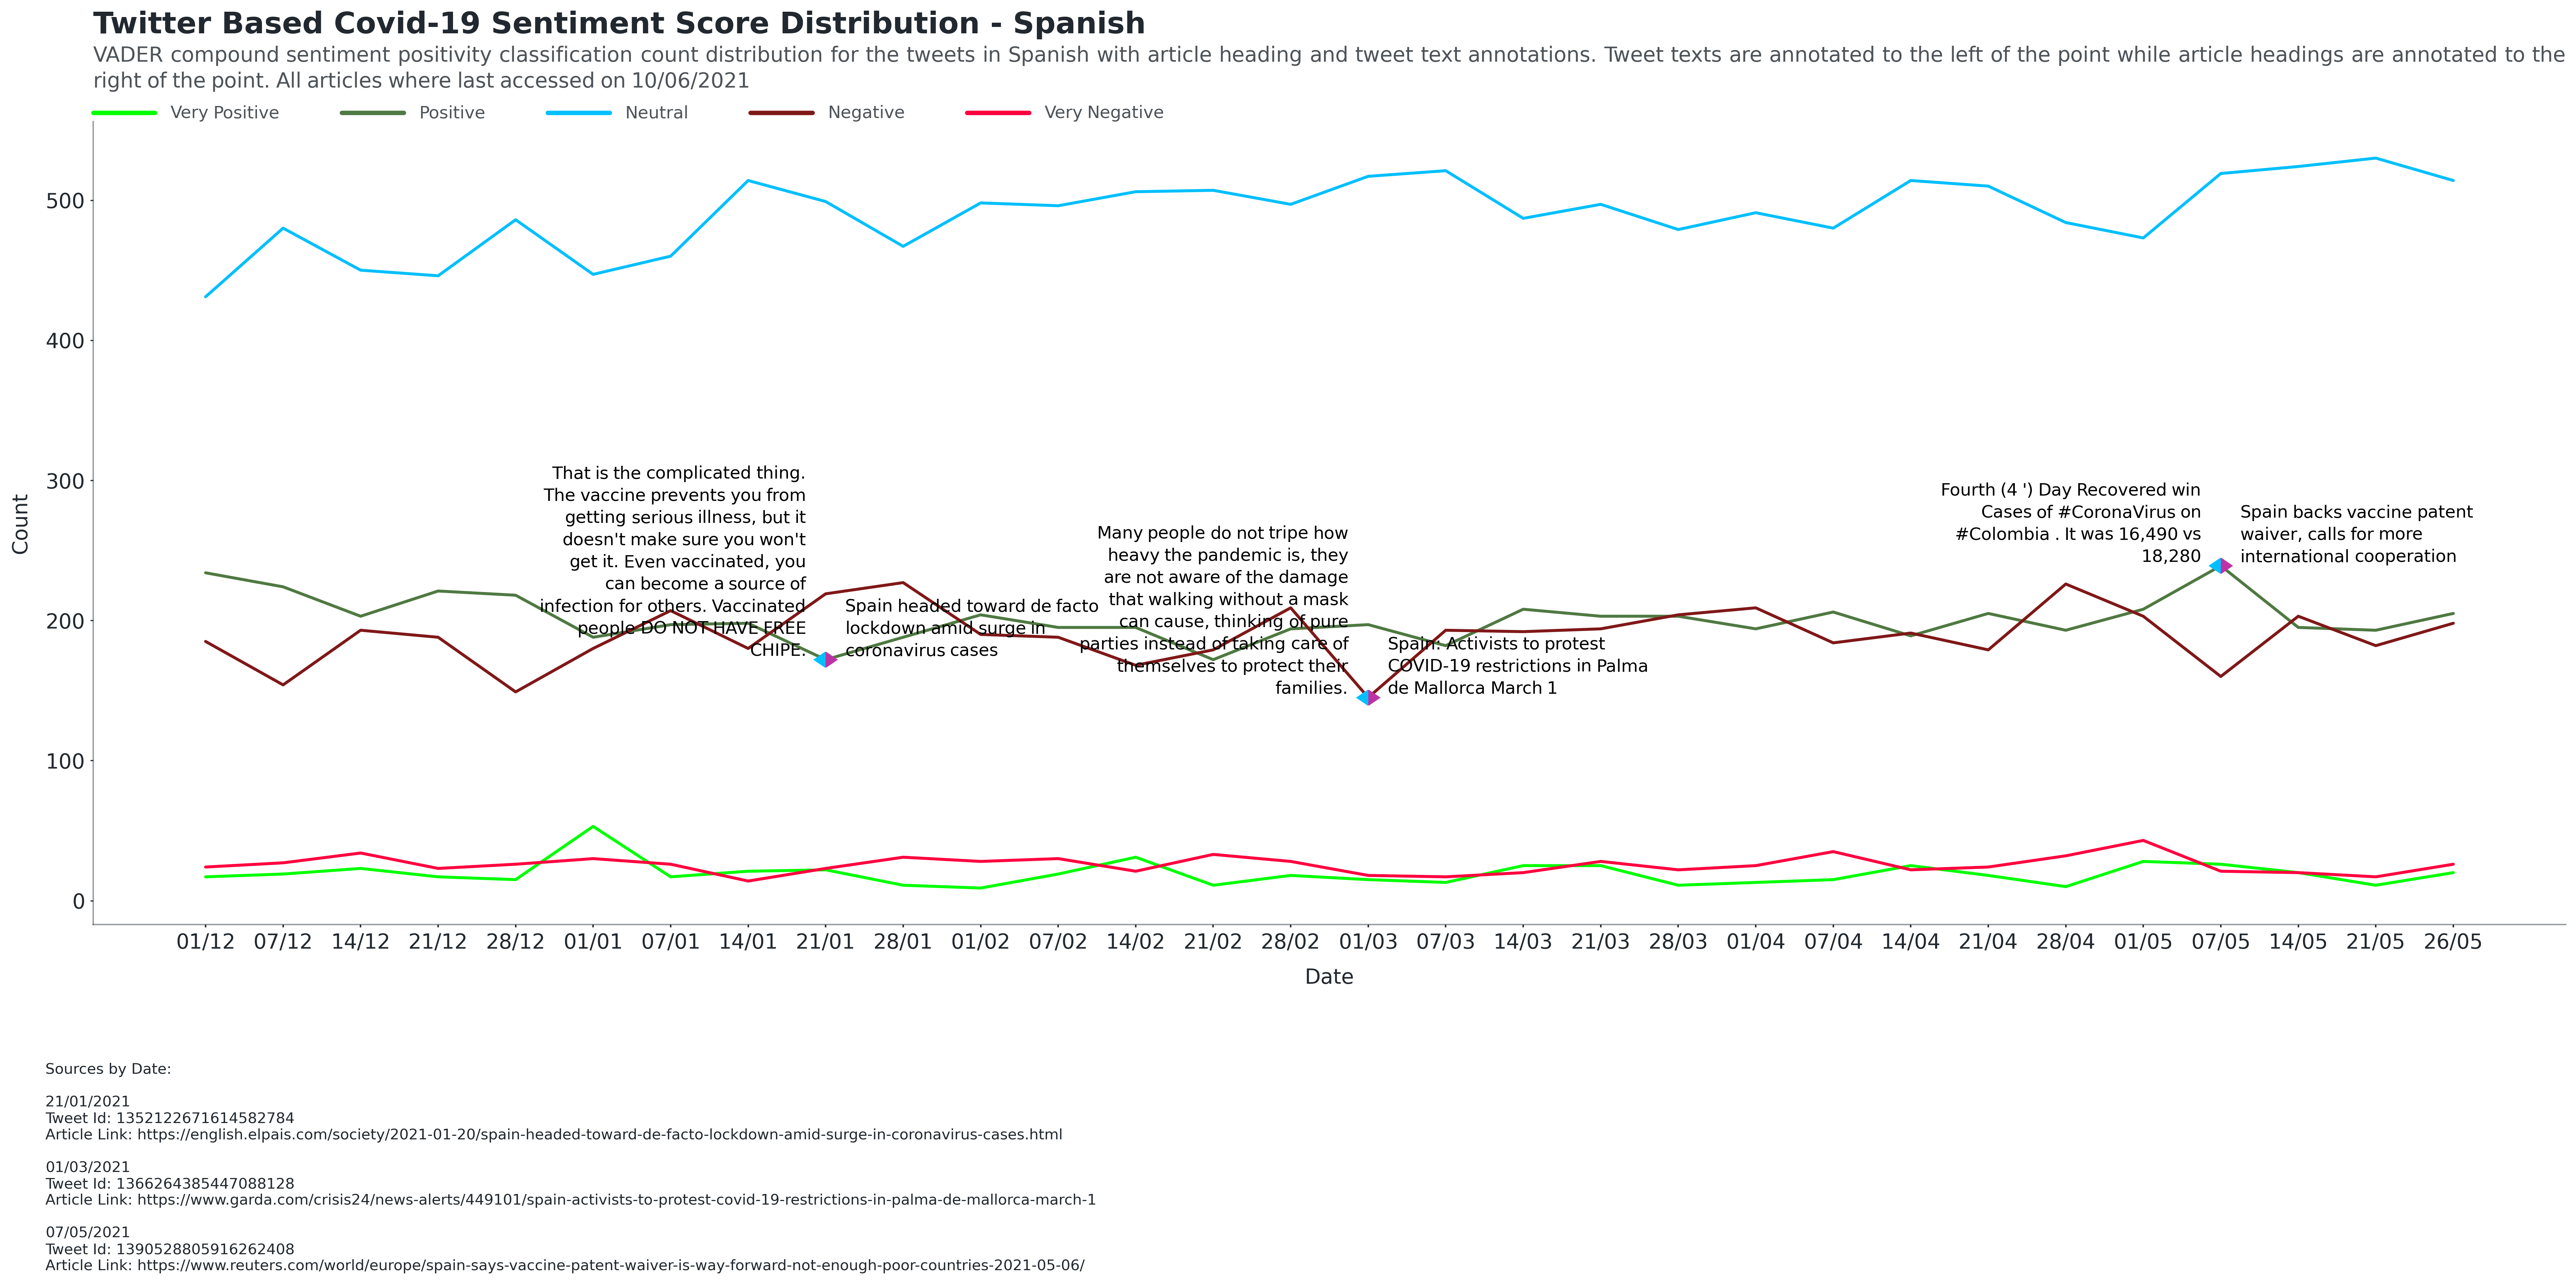
\includegraphics[scale=0.24]{Final Spanish Annotated Distribution.png}
%%\caption[English Annotated Sentiment Distribution]{ }
%%\label{fig:Spanish}
%%\end{figure}
%%
%%\noindent For figure~\ref{fig:Spanish}
%%
%%\begin{figure}[h!]
%%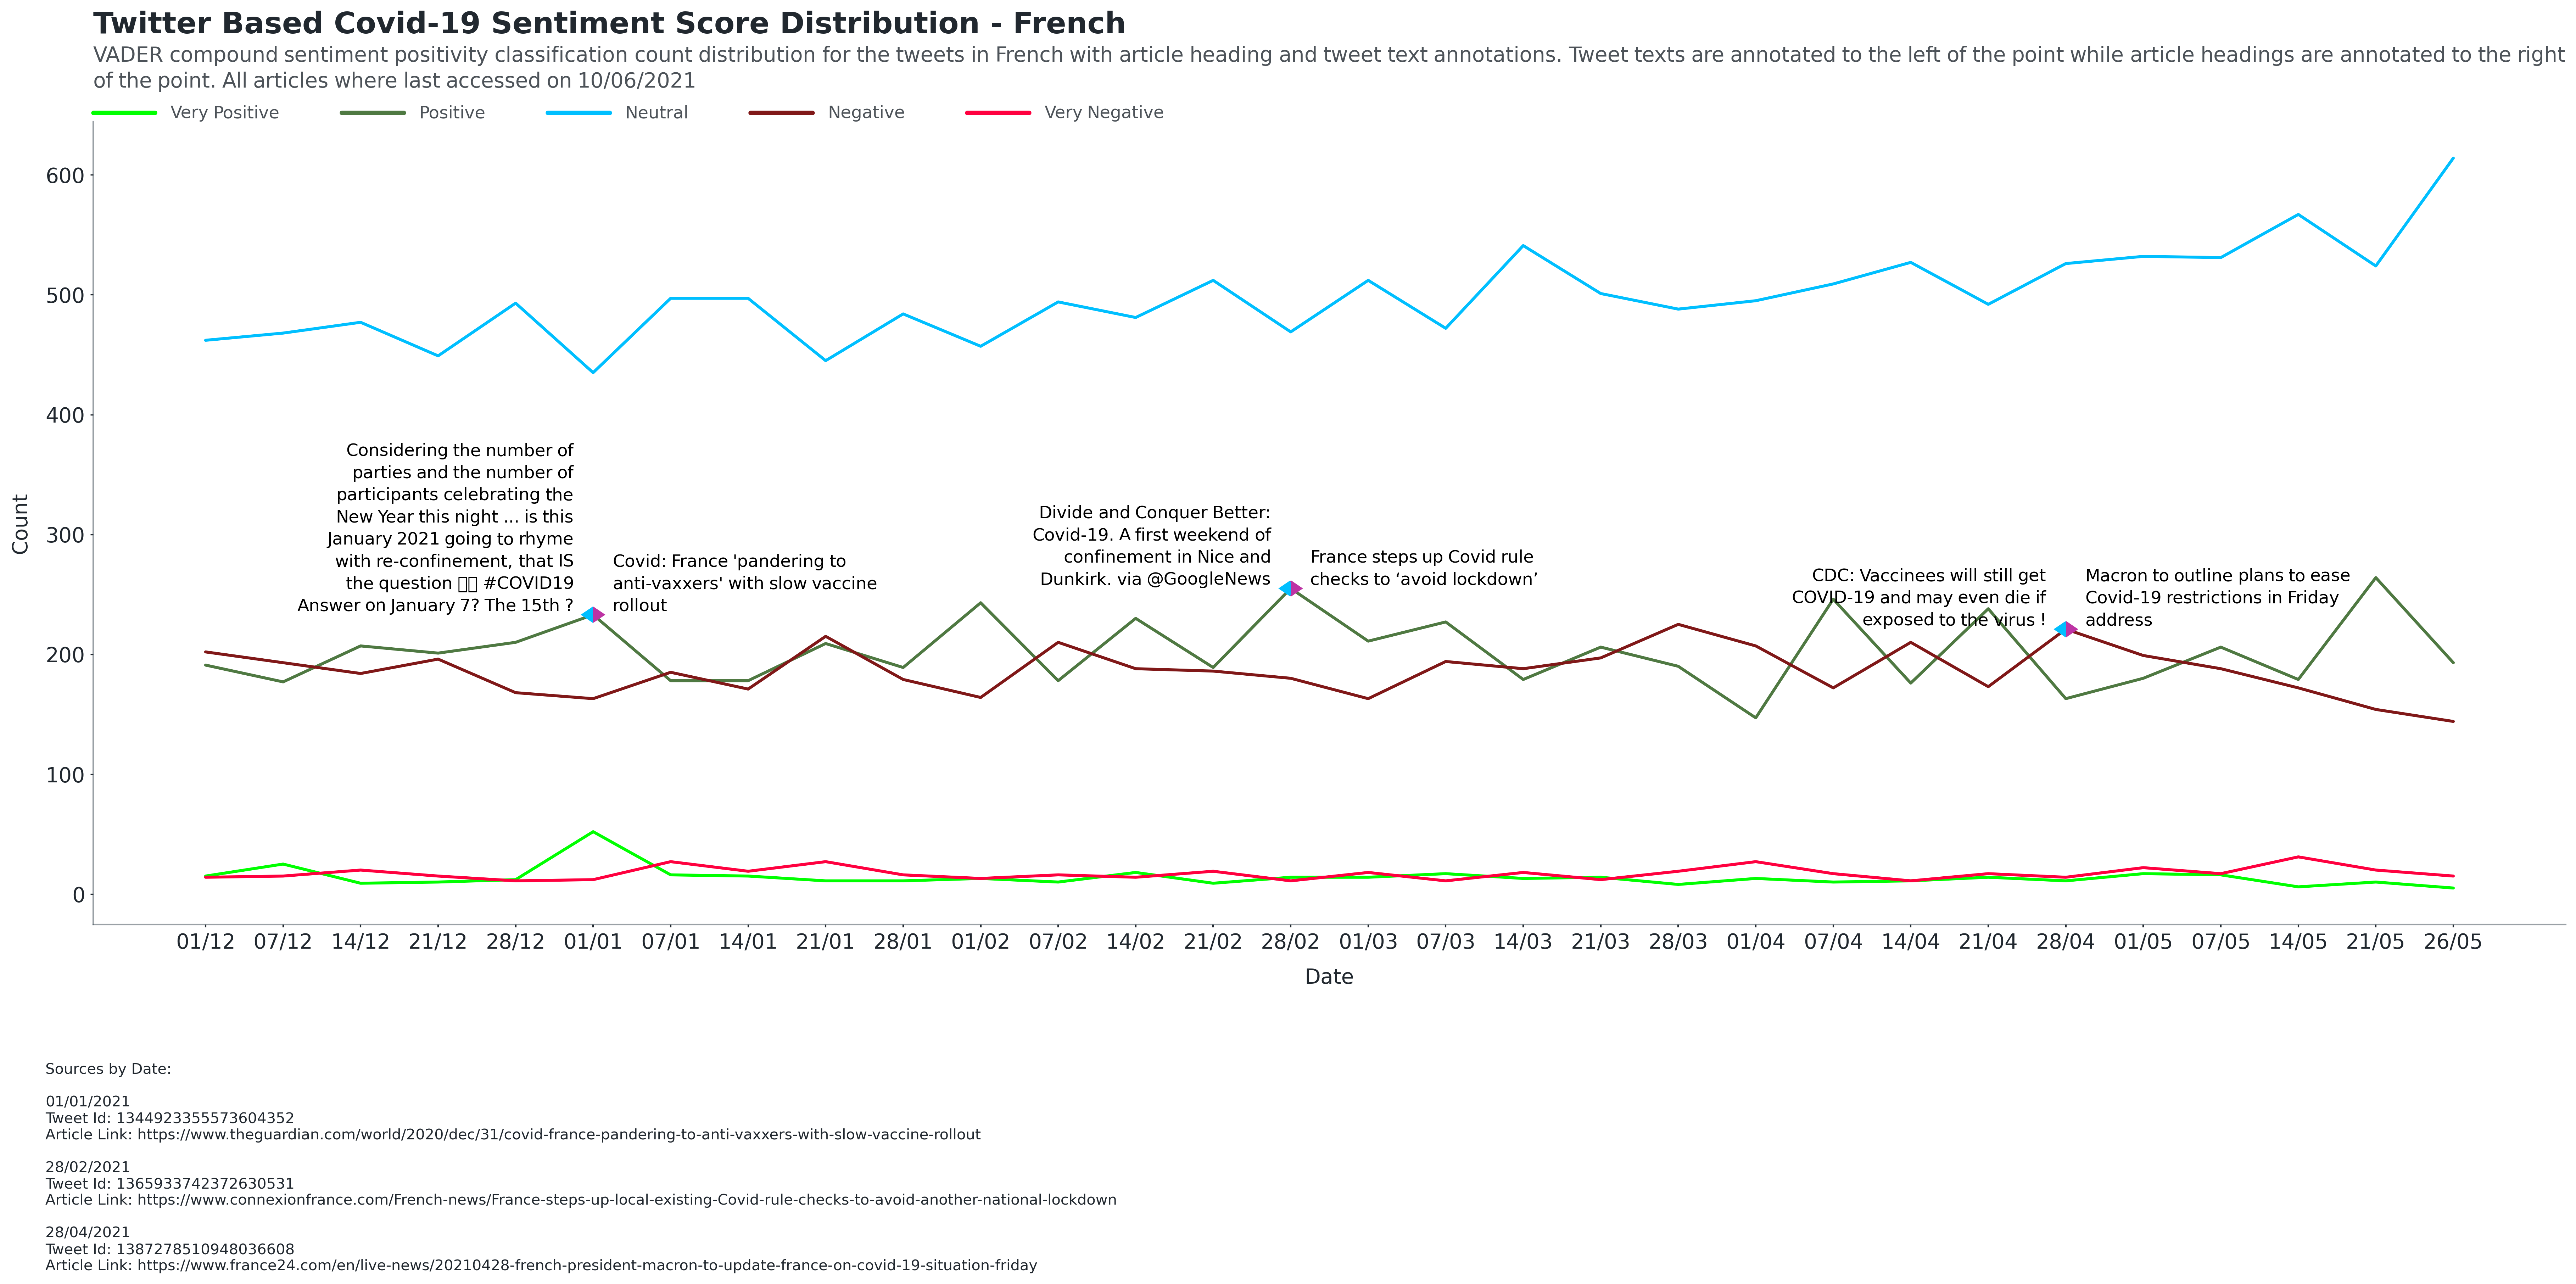
\includegraphics[scale=0.24]{Final French Annotated Distribution.png}
%%\caption[Final French Annotated Distribution]{ }
%%\label{fig:French}
%%\end{figure}
%%
%%\noindent For figure~\ref{fig:French}
%%
%%\begin{figure}[h!]
%%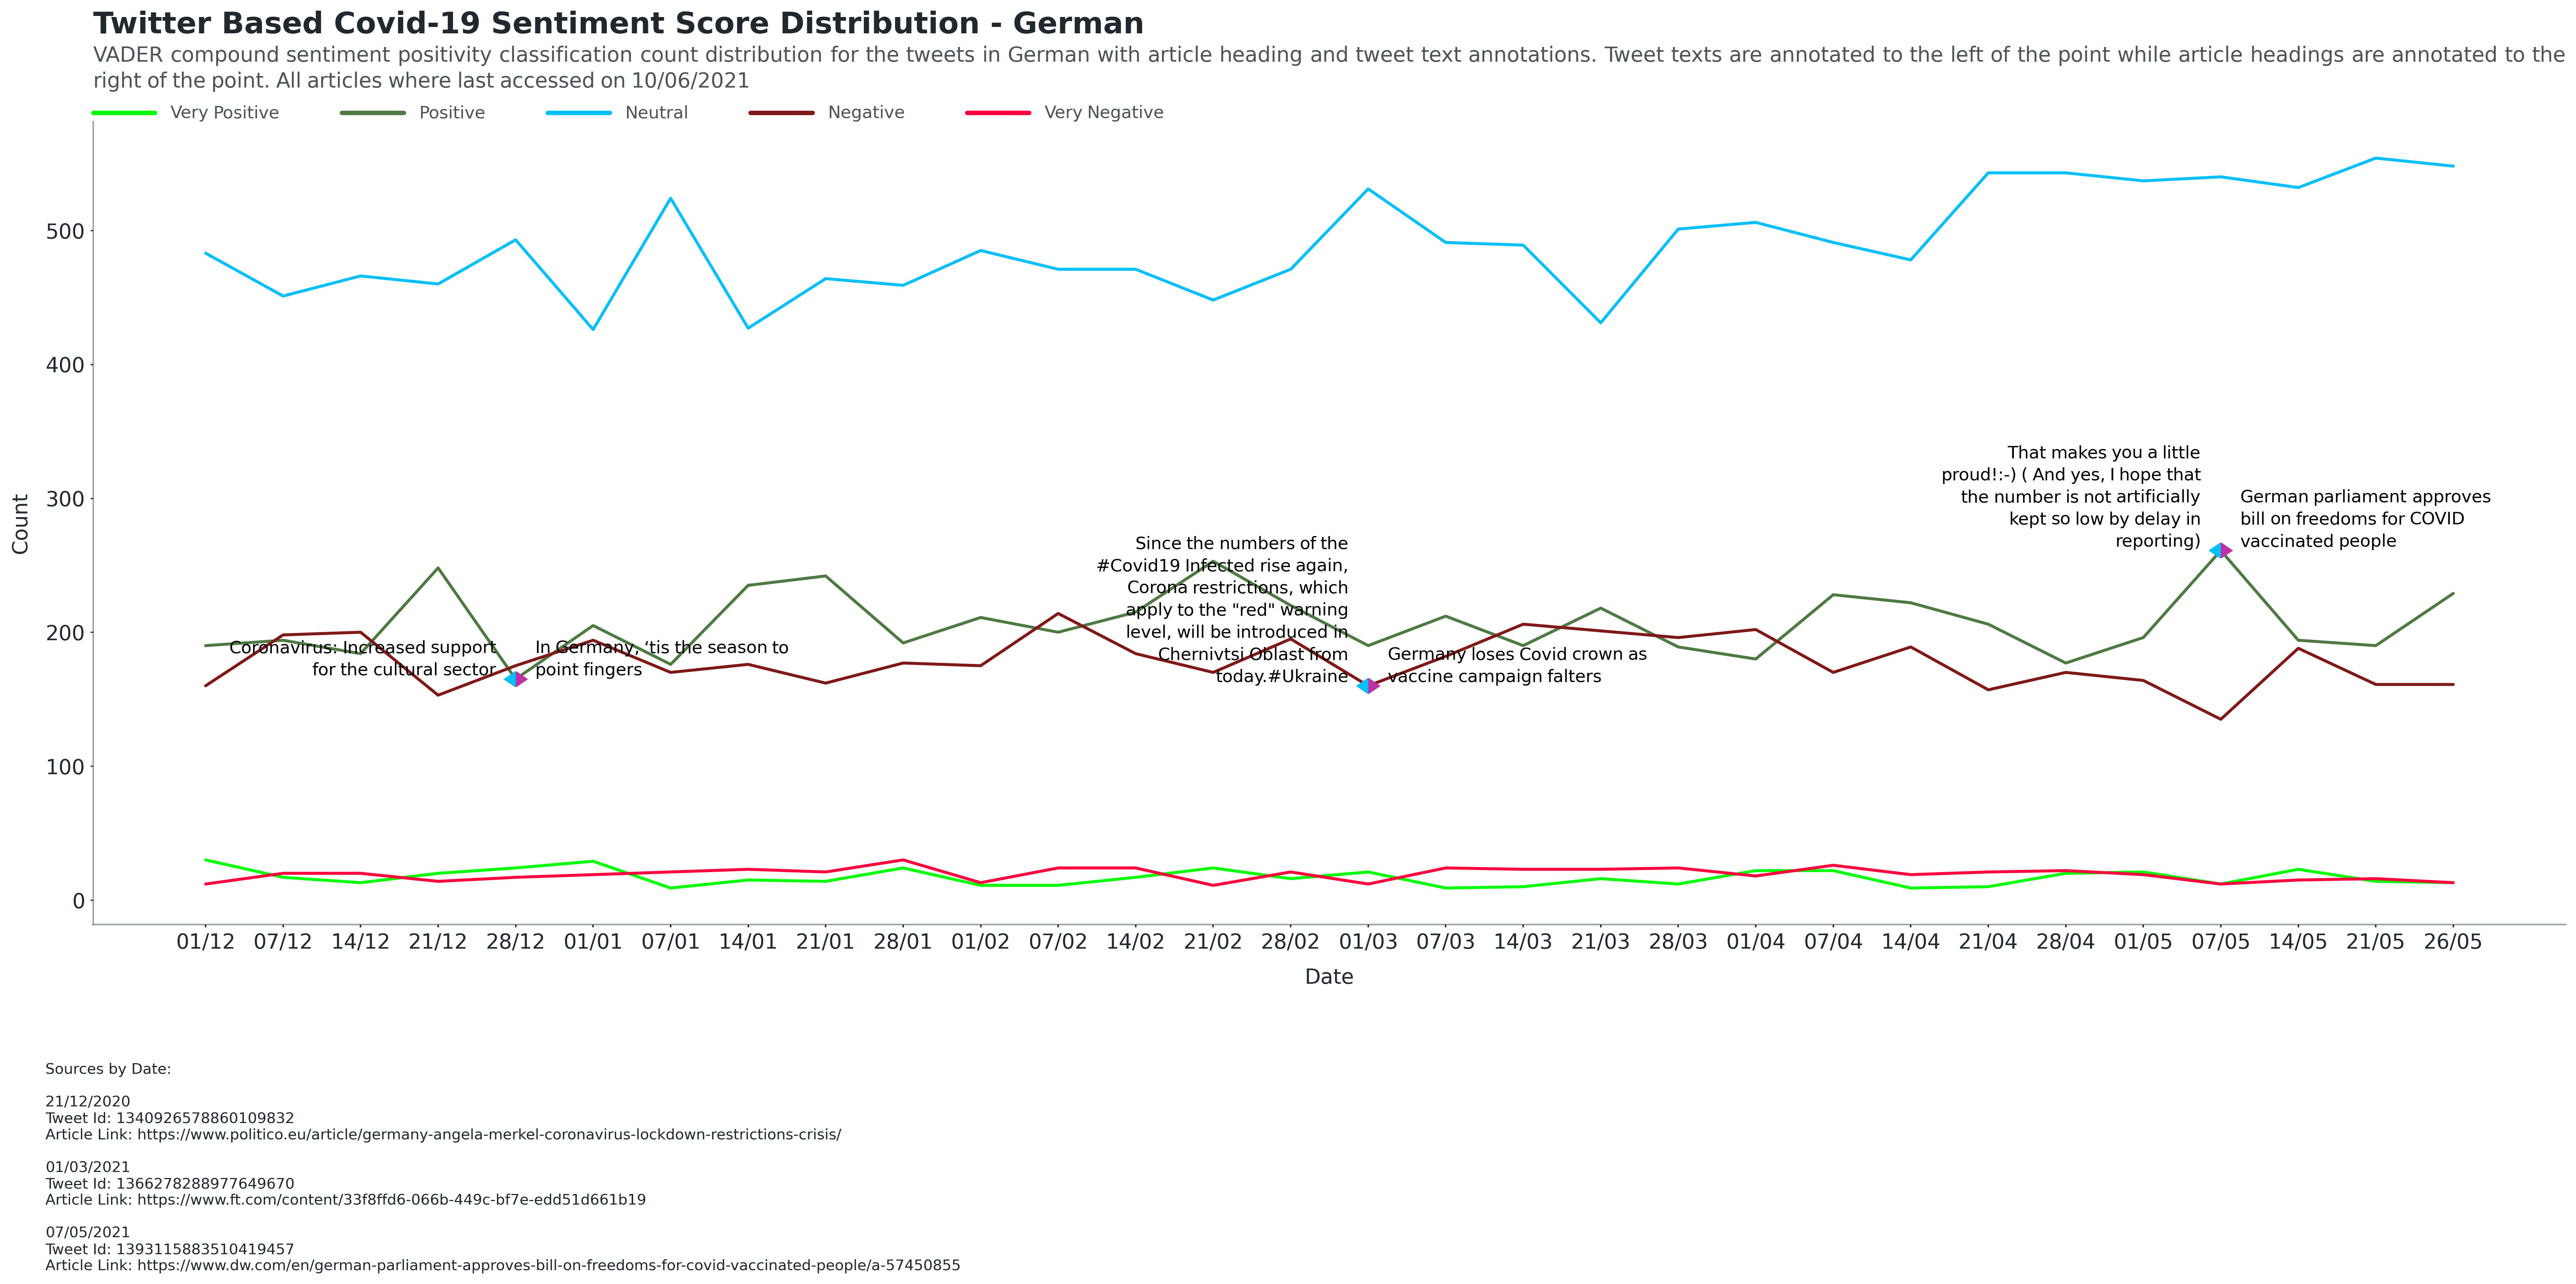
\includegraphics[scale=0.24]{Final German Annotated Distribution.png}
%%\caption[Final German Annotated Distribution]{ }
%%\label{fig:German}
%%\end{figure}
%%
%%\noindent For figure~\ref{fig:German}
%%
%%\begin{figure}[h!]
%%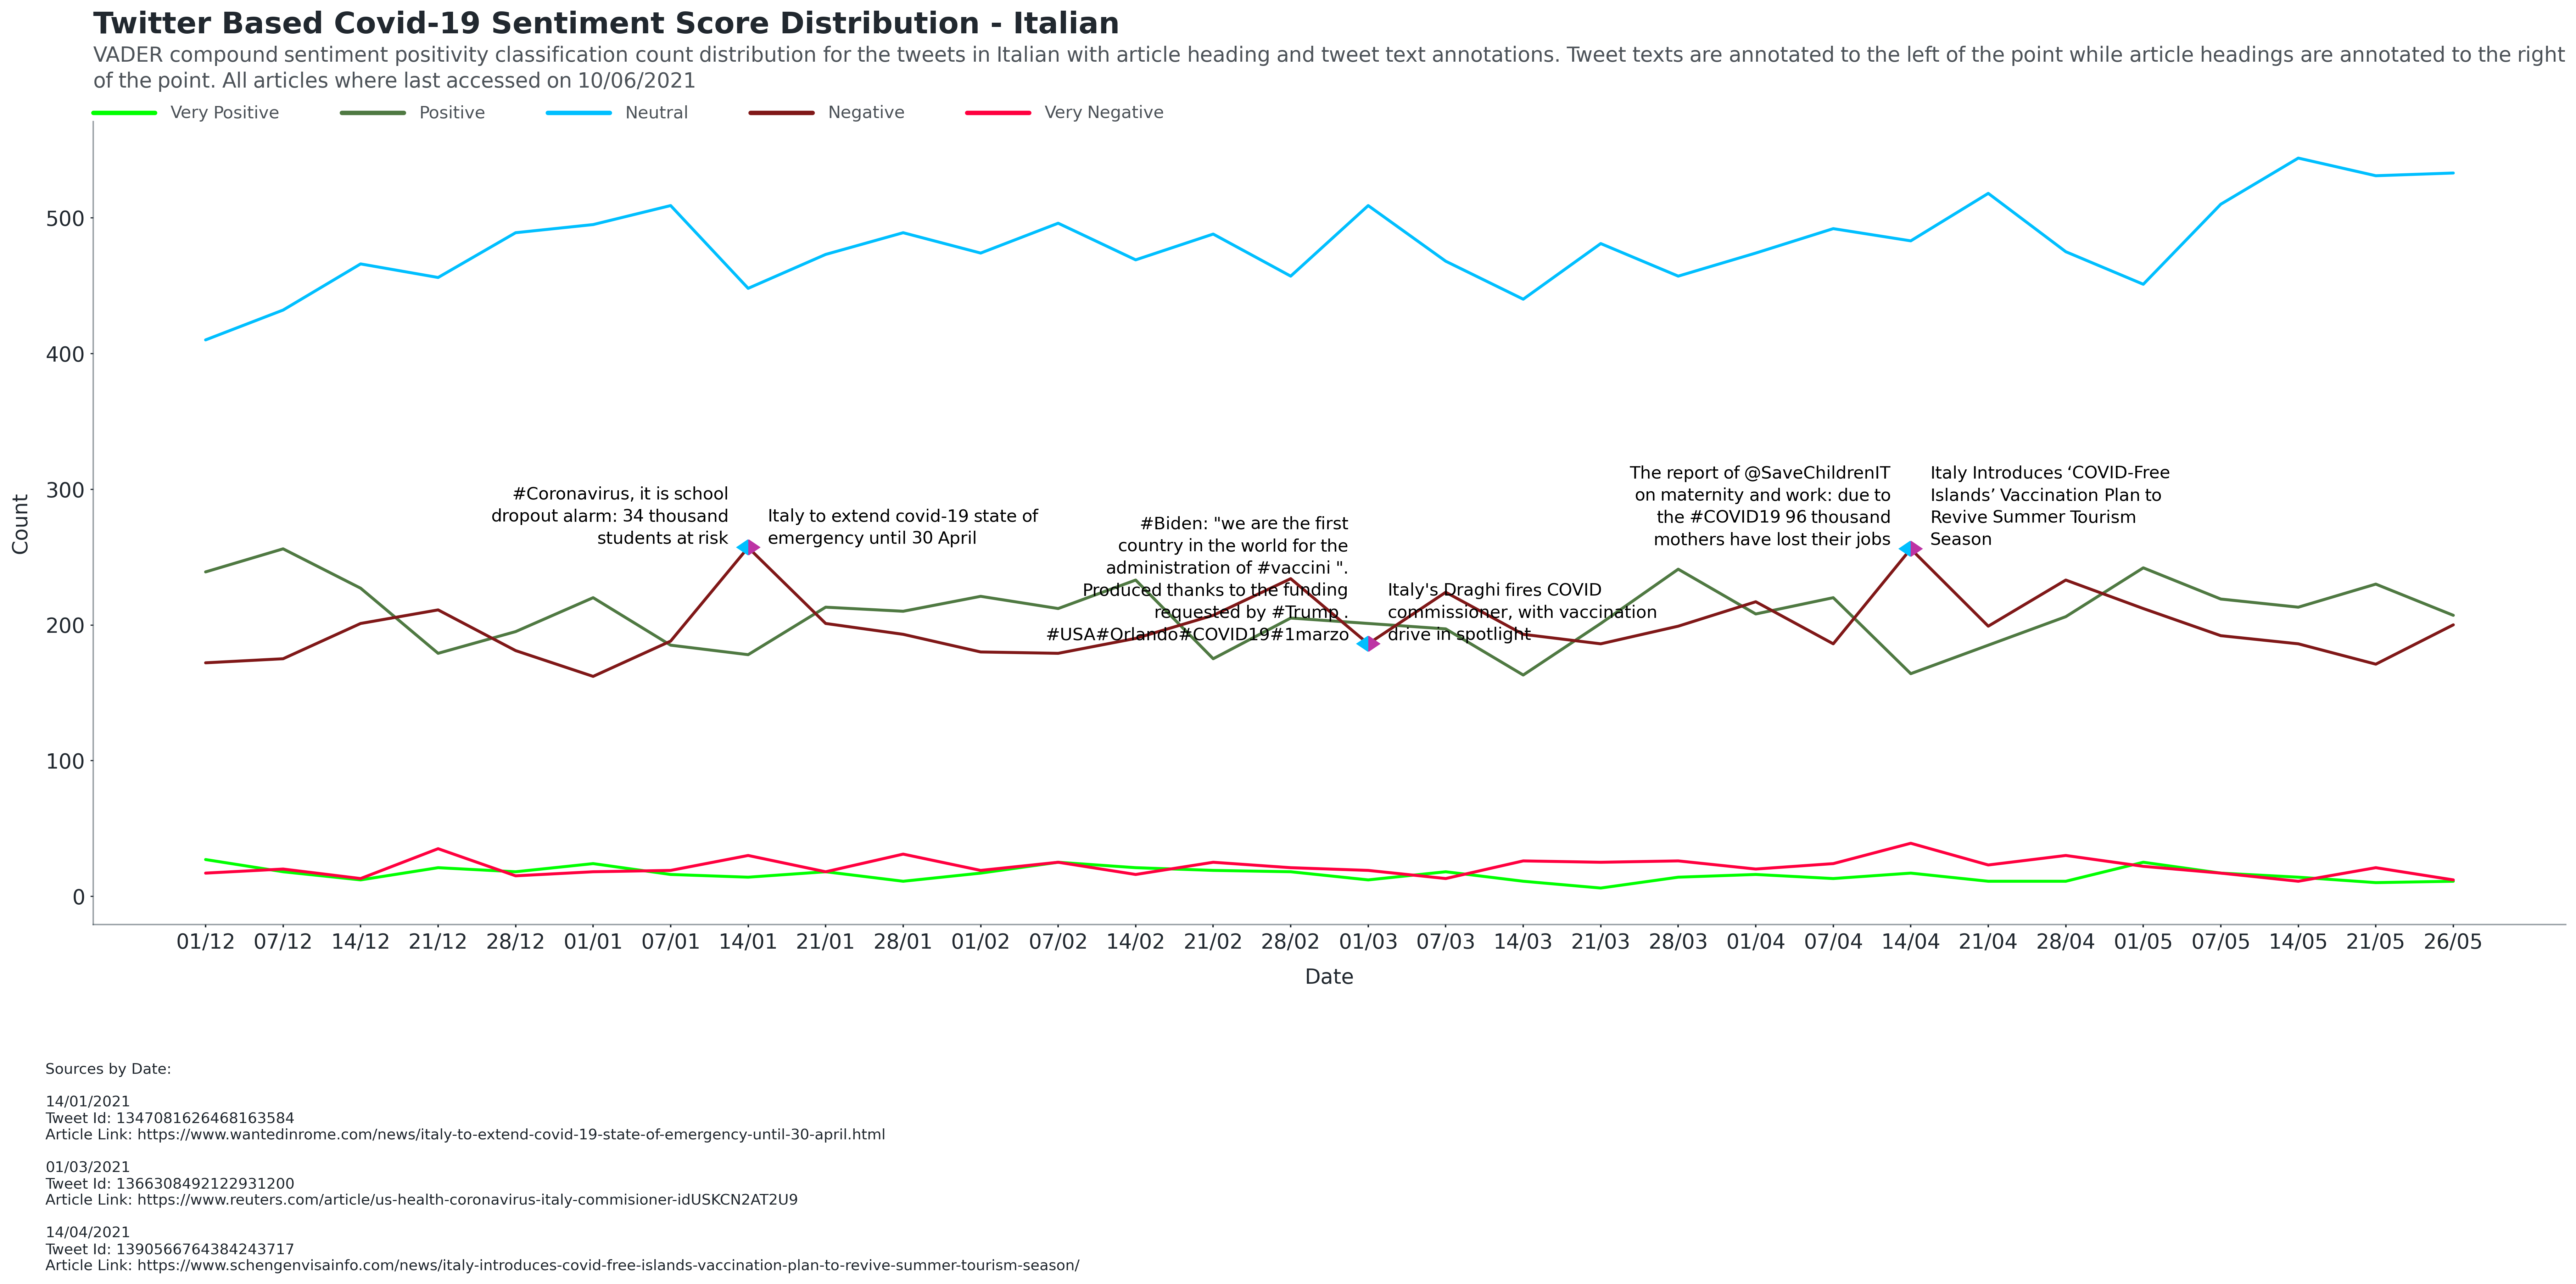
\includegraphics[scale=0.24]{Final Italian Annotated Distribution.png}
%%\caption[Final Italian Annotated Distribution]{ }
%%\label{fig:Italian}
%%\end{figure}
%%
%%\noindent For figure~\ref{fig:Italian}
%%
%%\begin{figure}[h!]
%%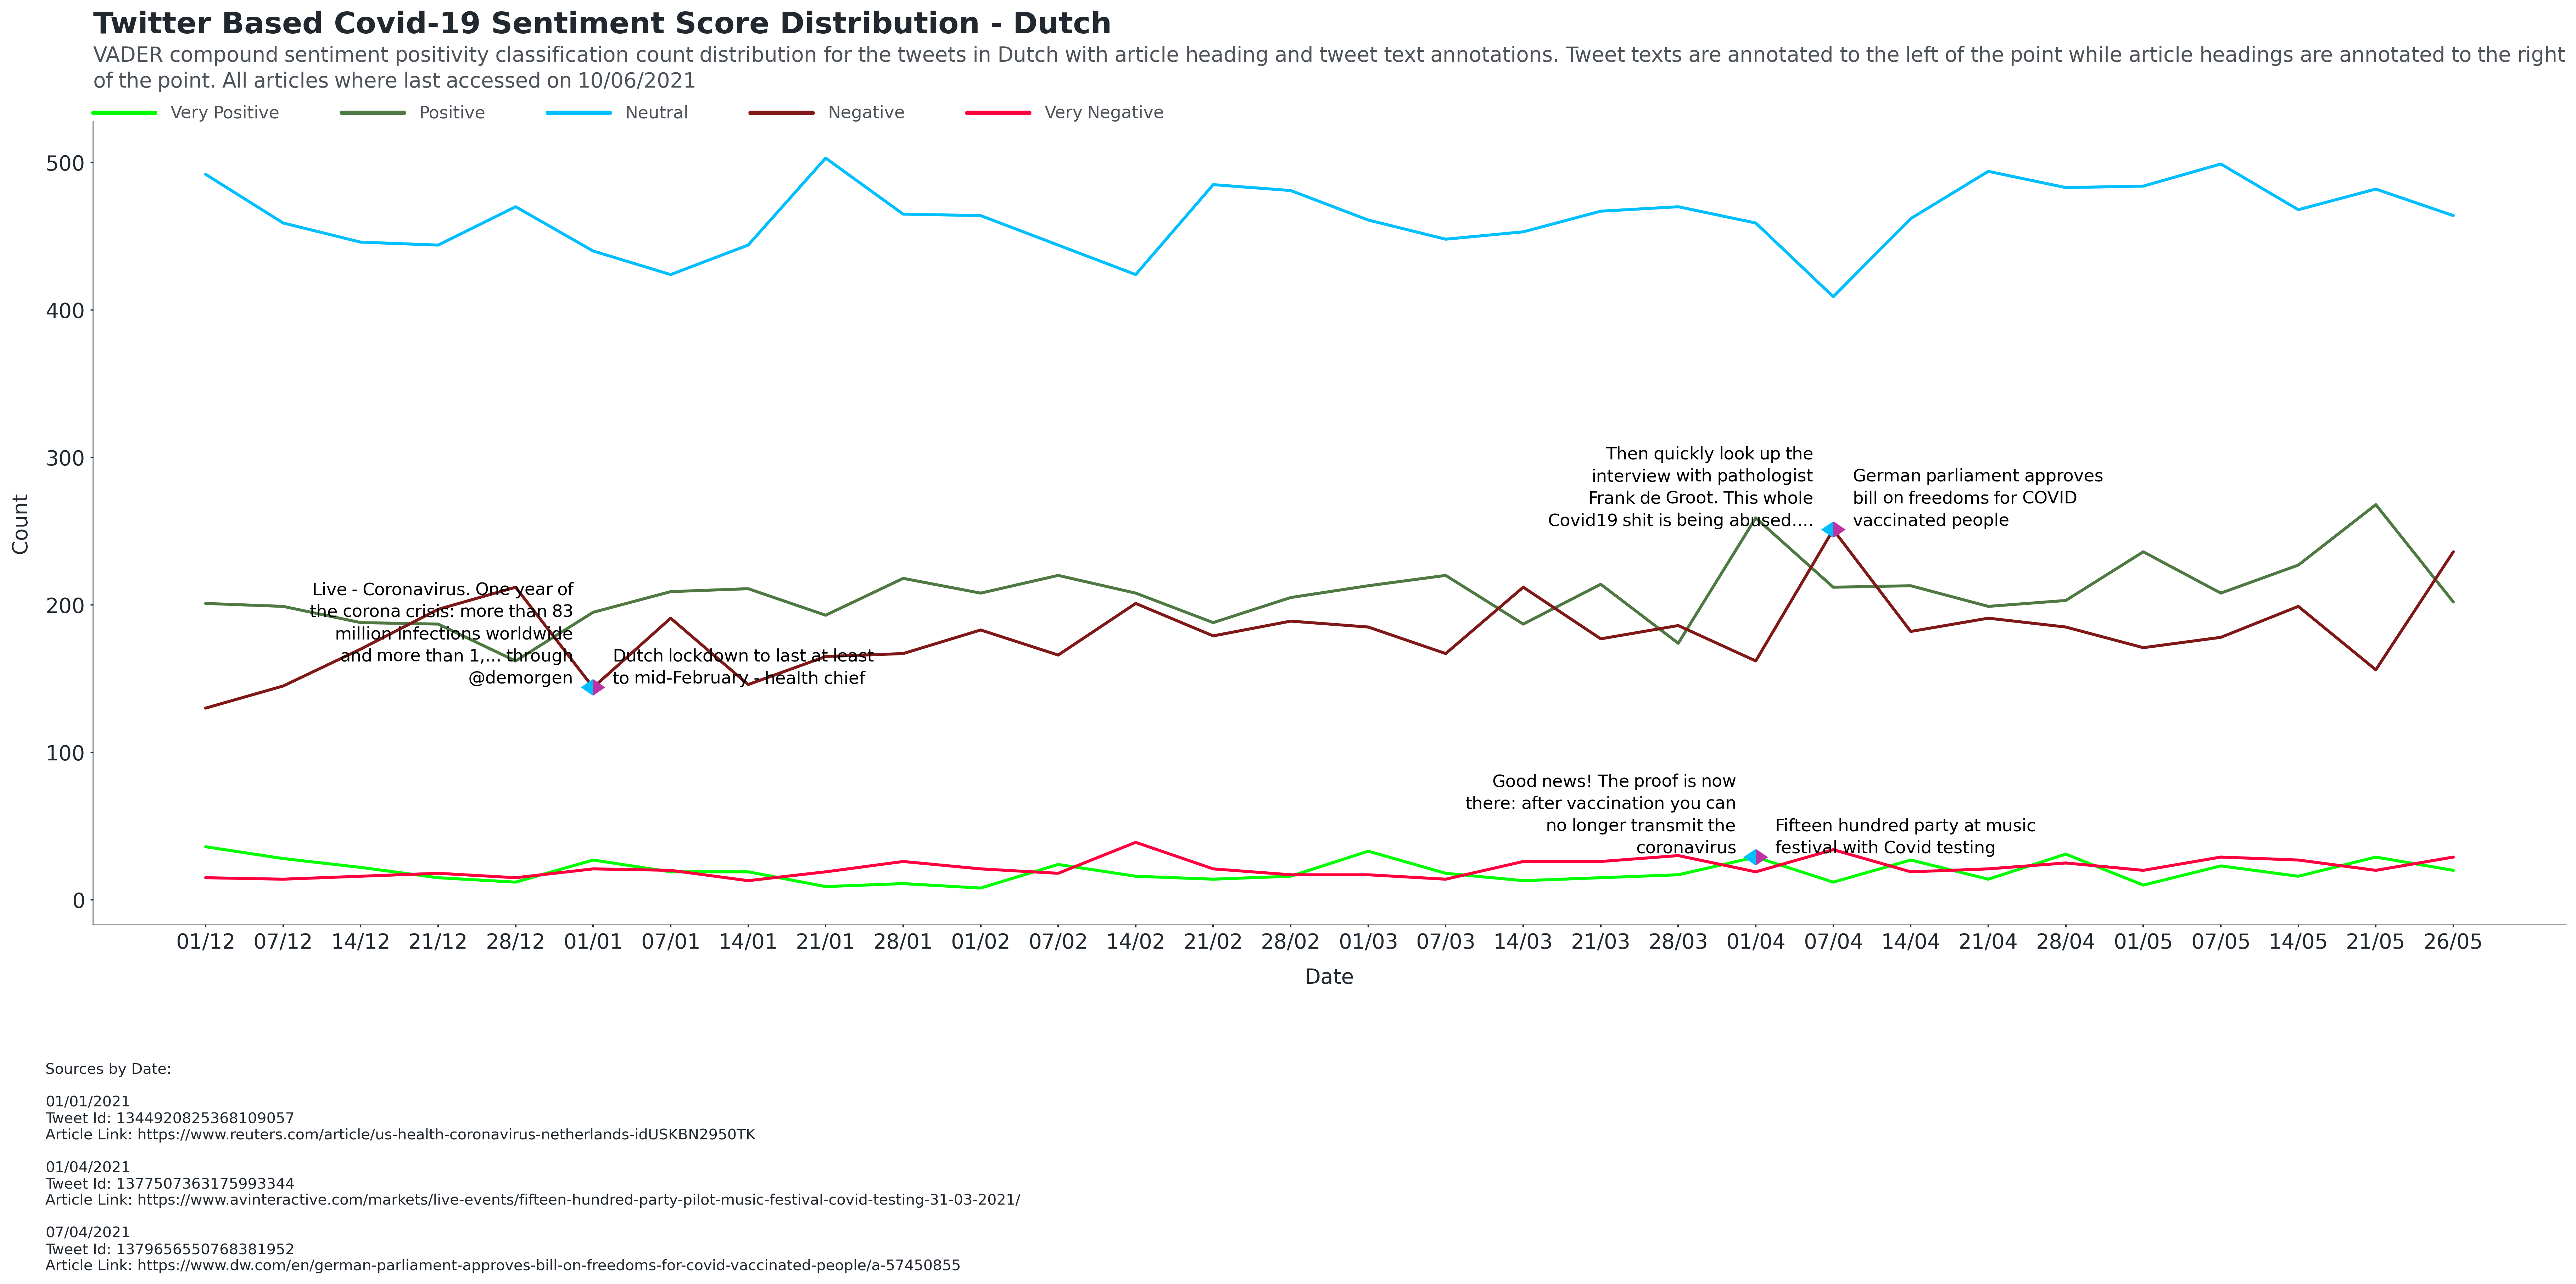
\includegraphics[scale=0.24]{Final Dutch Annotated Distribution.png}
%%\caption[Final Dutch Annotated Distribution]{ }
%%\label{fig:Dutch}
%%\end{figure}
%%
%%\noindent For figure~\ref{fig:Dutch}
%
%\section{Daily Article vs Twitter Mean Sentiment}
%
%To see the relationship news articles and tweets have the daily mean sentiment scores of each language where plotted.
%In figure~\ref{fig:artcilevstwitter} a clear relationship can be seen between the two datasets.
%When one goes down so does the other, and vice-versa.
%The values for the article dataset carry more information since the dataset is smaller and is guaranteed to be on topic.
%
%\begin{figure}[h!]
%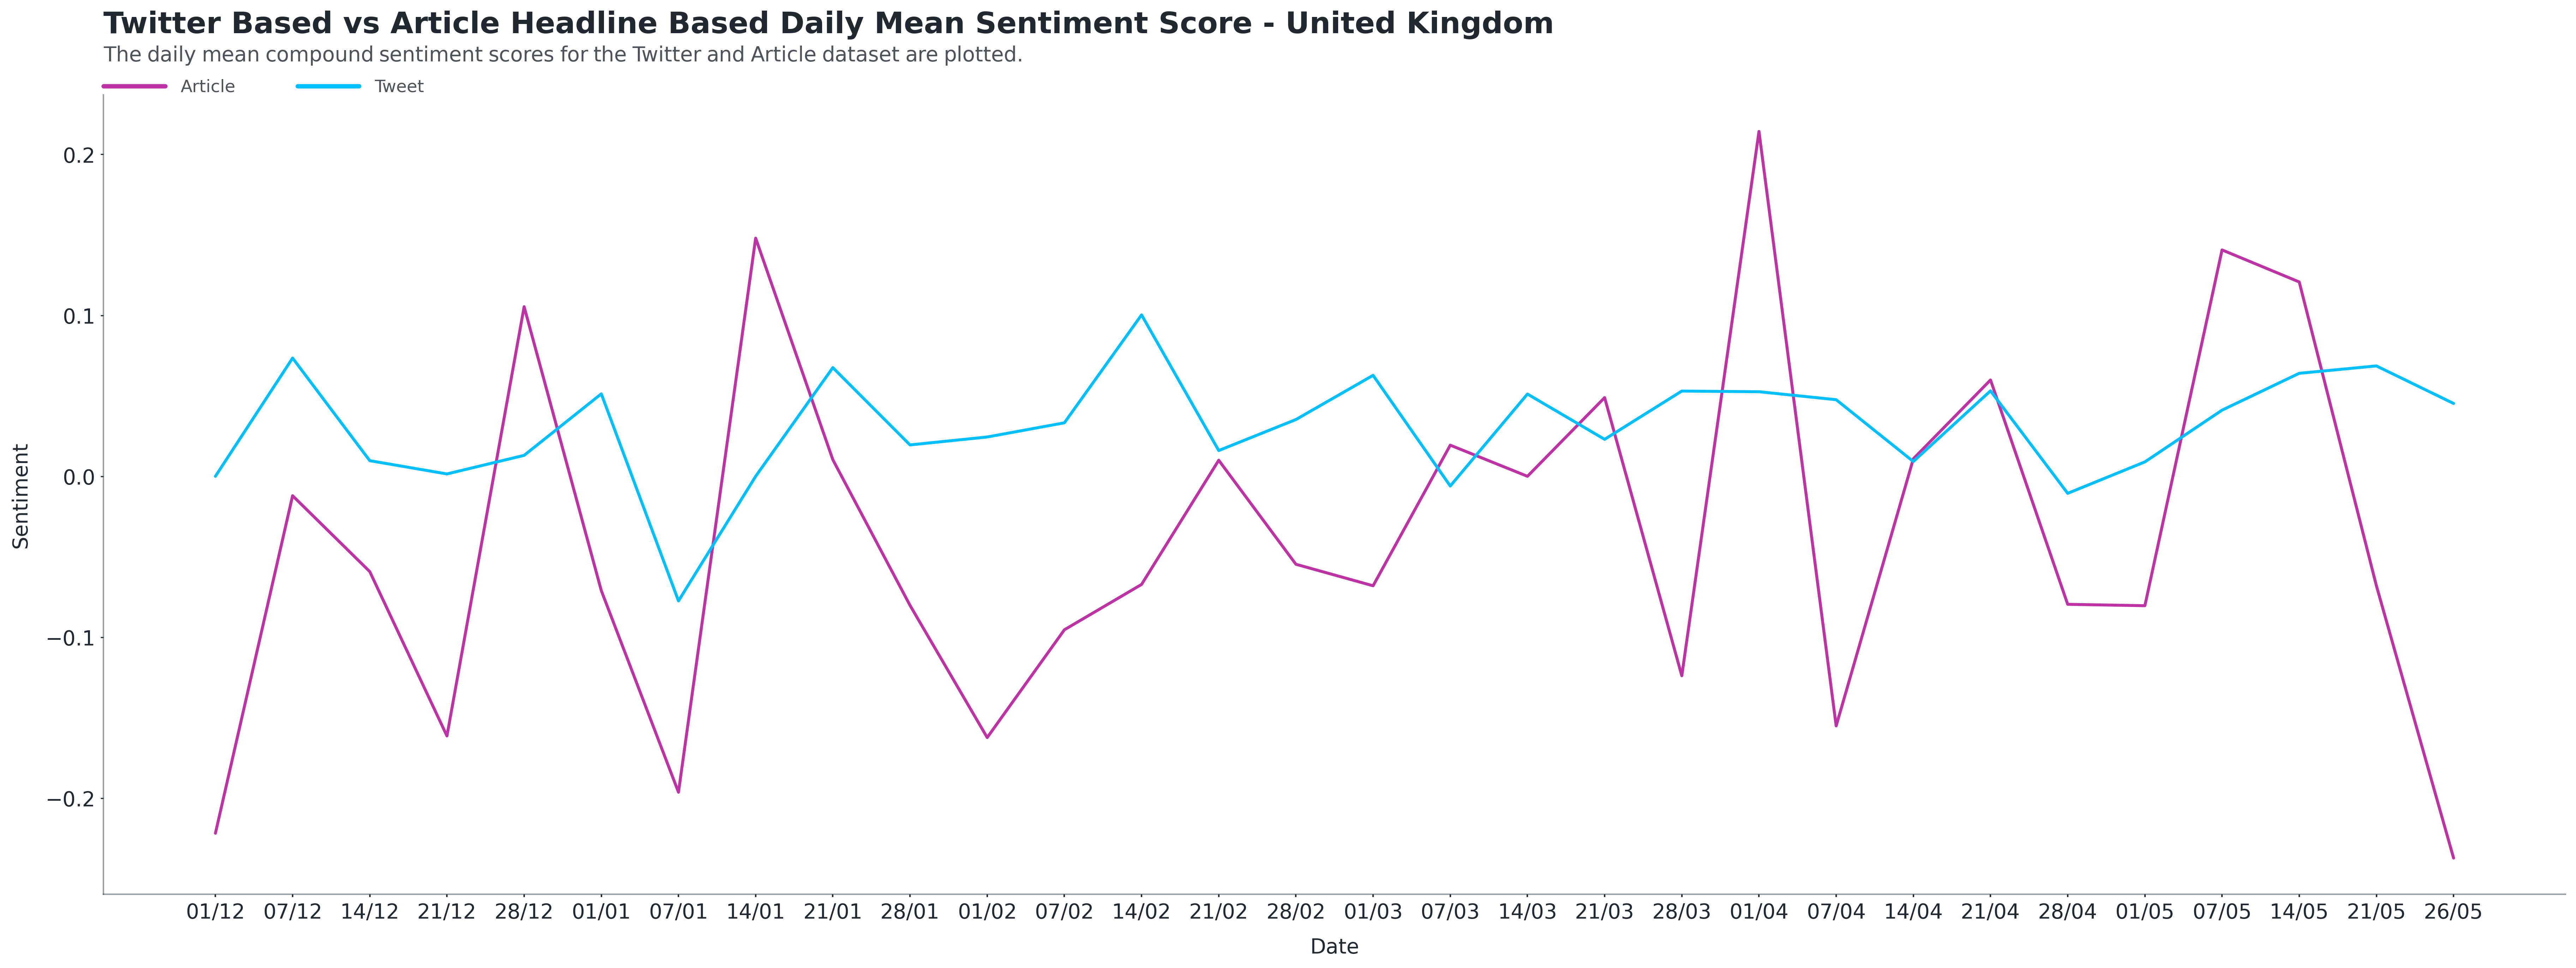
\includegraphics[scale=0.24]{Daily Mean Article VS Twitter UK.png}
%\caption[Daily Mean Article VS Twitter]{ }
%\label{fig:artcilevstwitter}
%\end{figure}
%
%\section{Word Frequency in the Form of Word Clouds}
%
%Finally the a word cloud was generated for each month in each language.
%These word clouds where used to follow the difference of word usage over the 6 month period.
%Figures~\ref{fig:frdec} to ~\ref{fig:frmay} follow the French tweets.
%
%\begin{figure}[!htb]
%\minipage{0.33\textwidth}
%  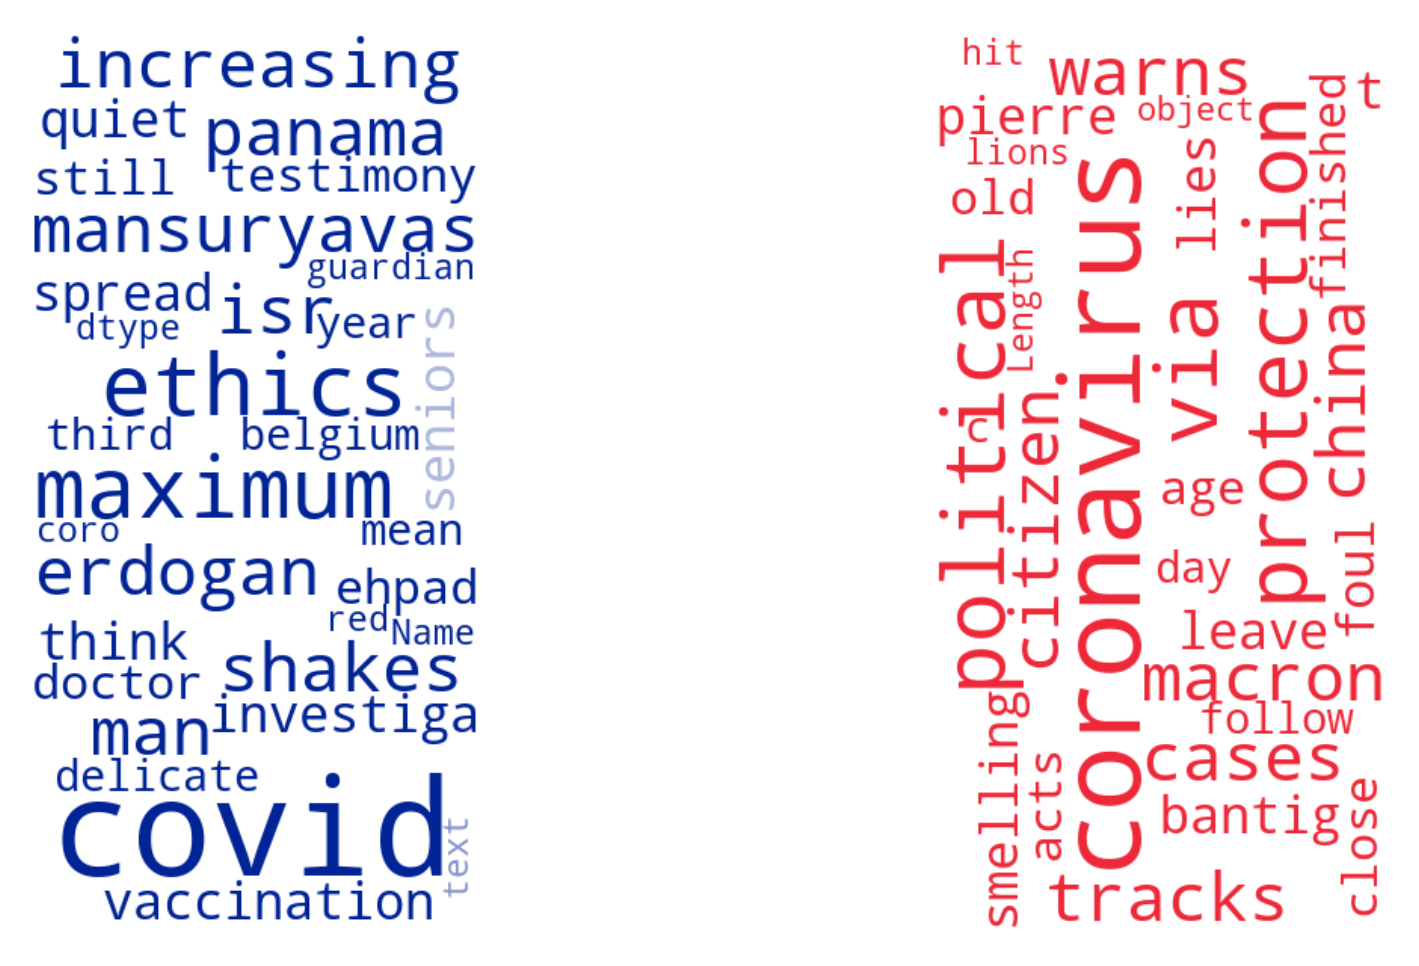
\includegraphics[width=\linewidth]{December fr word cloud.png}
%  \caption[French word cloud for December]{December}\label{fig:frdec}
%\endminipage\hfill
%\minipage{0.33\textwidth}
%  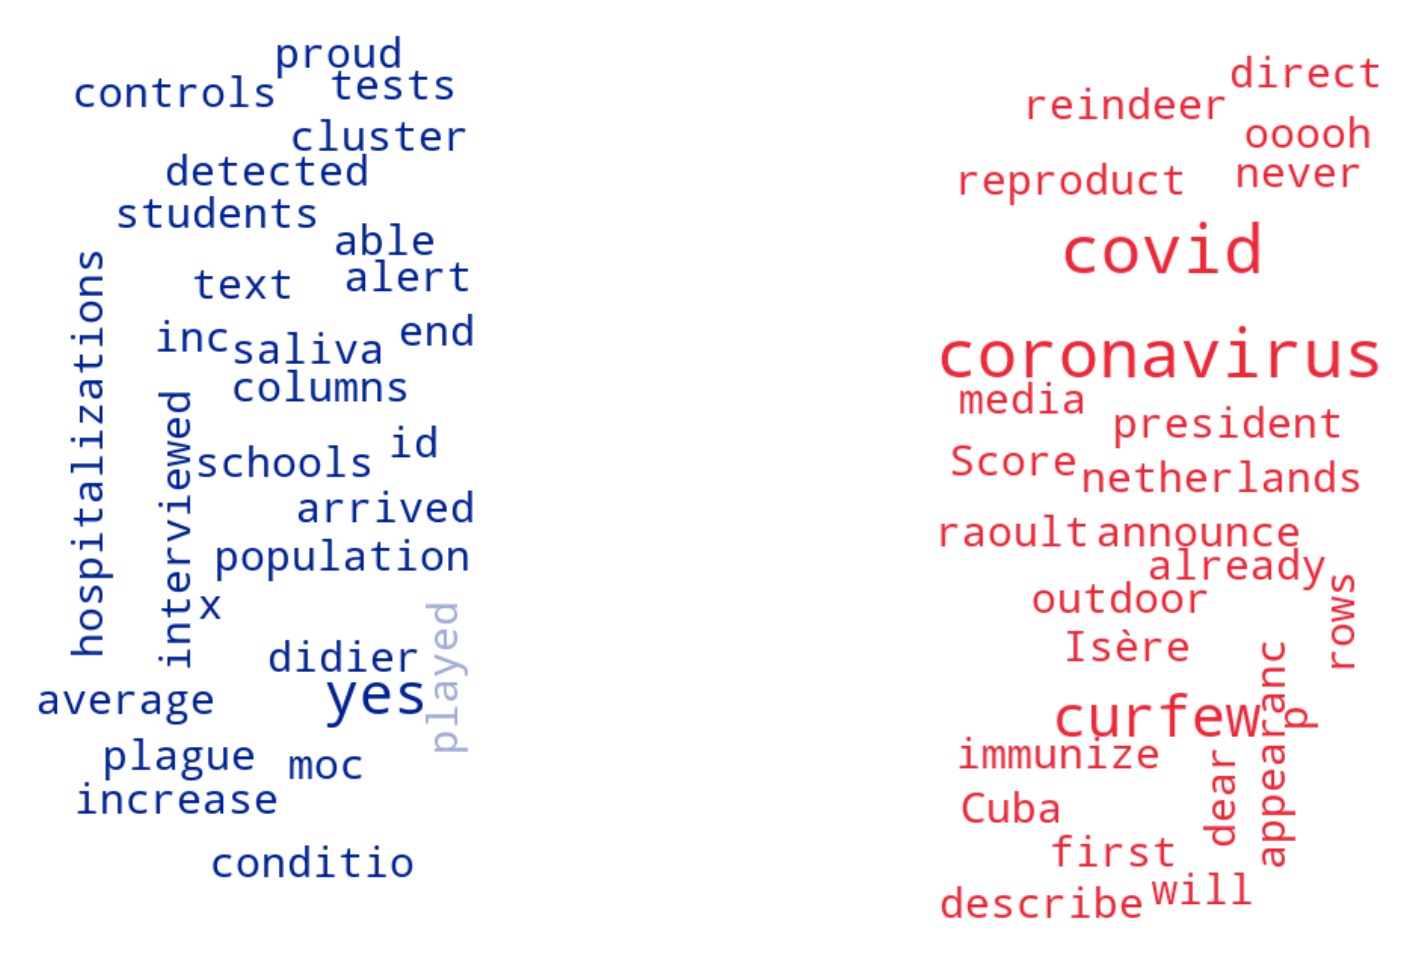
\includegraphics[width=\linewidth]{February fr word cloud.png}
%  \caption[French Word cloud for February]{February}\label{fig:frfeb}
%\endminipage\hfill
%\minipage{0.33\textwidth}
%  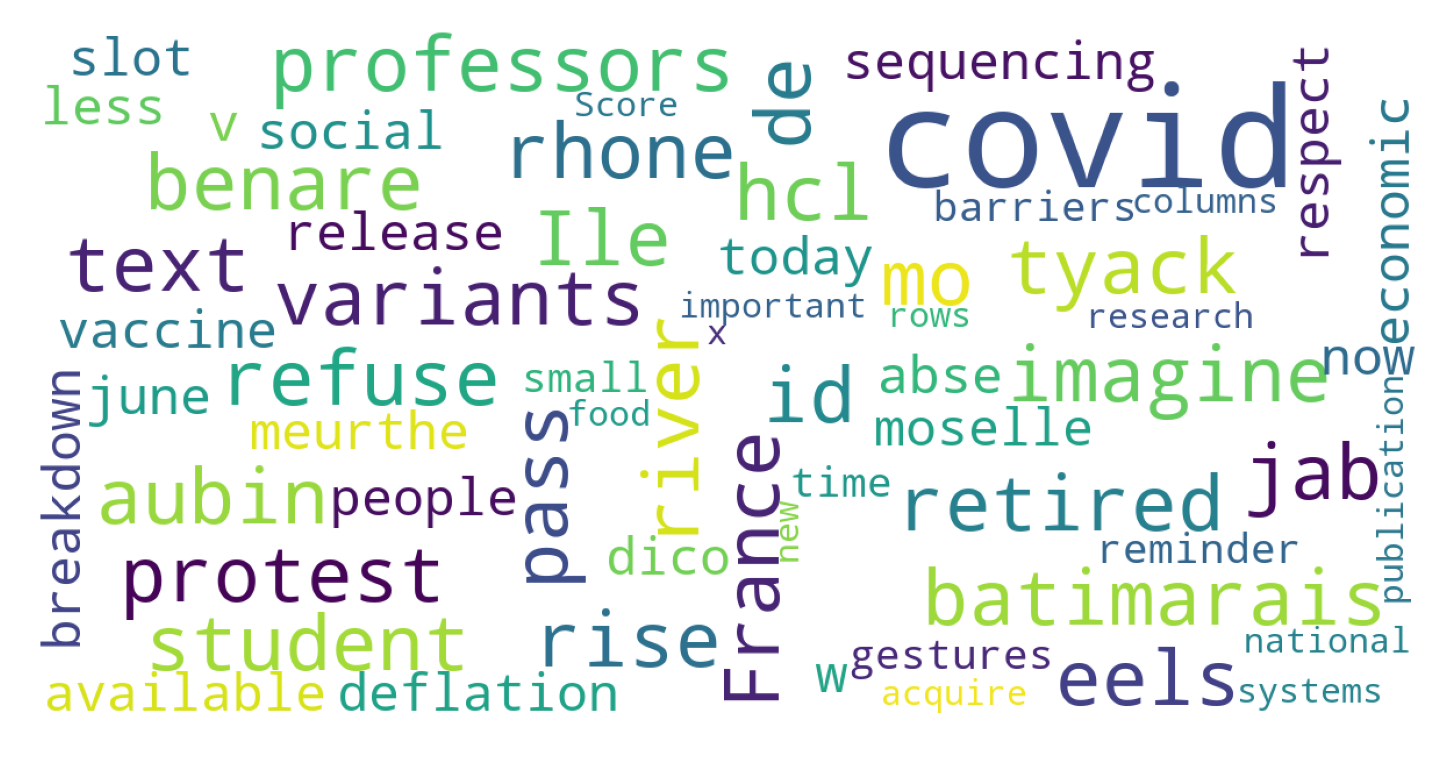
\includegraphics[width=\linewidth]{May fr word cloud.png}
%  \caption[French Word cloud for May]{May}\label{fig:frmay}
%\endminipage
%\end{figure}
